% DH607 project report, a standalone document.
% Every number is from docs/submission/paper.tex, docs/submission/partA.tex
% and the development notes as of 24 November 2026.
% Build: latexmk -pdf report.tex
\documentclass[11pt]{article}

\newcommand{\myname}{Nirav Bhattad}
\newcommand{\myrollnumber}{23B3307}
\newcommand{\topicname}{PhaseBudget: which reads to keep, and when to trust a phase}

\usepackage{nirav}
\usetikzlibrary{arrows.meta,positioning,calc,shapes.geometric}
\usepackage{pgfplots}
\pgfplotsset{compat=1.18}
\lhead{\fontfamily{lmss}\selectfont PhaseBudget, DH607 report}
\usepackage{etoolbox}
\usepackage{multicol}
\usepackage{pifont,makecell}
% keep each code block on one page
\BeforeBeginEnvironment{lstlisting}{\par\noindent\begin{minipage}{\linewidth}}
\AfterEndEnvironment{lstlisting}{\end{minipage}\par}

\setlist[enumerate]{itemsep=0.3mm, topsep=0.5mm, leftmargin=*}
\setlist[itemize]{itemsep=0.3mm, topsep=0.5mm, leftmargin=*}
\lstset{language=Python, numbers=none, basicstyle=\footnotesize\ttfamily,
  aboveskip=3pt, belowskip=3pt, columns=fullflexible, keepspaces=true, upquote=true}

\newcommand{\code}[1]{\texttt{#1}}
\newcommand{\dna}[1]{\texttt{#1}}
\newcommand{\grp}[1]{\texttt{#1}}
\newcommand{\Bin}{\mathrm{Bin}}
\definecolor{keep}{HTML}{1F77B4}
\definecolor{drop}{HTML}{C8C8C8}
\definecolor{good}{HTML}{2CA02C}
\definecolor{bad}{HTML}{D62728}
\definecolor{hapA}{HTML}{1F77B4}
\definecolor{hapB}{HTML}{D62728}

\tikzset{
  box/.style={draw,rounded corners=2pt,align=center,font=\footnotesize,
    inner sep=3pt,fill=gray!6,minimum height=7mm},
  hl/.style={box,fill=orange!15,draw=orange!80!black,thick},
  dec/.style={draw,diamond,aspect=2.2,align=center,font=\footnotesize,
    inner sep=1pt,fill=blue!5},
  arr/.style={-{Stealth},thick},
}

% Horizontal bar: y, label, fraction, count text, colour.
\newcommand{\failbar}[5]{%
  \node[anchor=east,font=\scriptsize,align=right] at (-0.03,#1) {#2};
  \fill[gray!20] (0,#1-0.13) rectangle (1,#1+0.13);
  \fill[#5] (0,#1-0.13) rectangle ({max(#3,0.008)},#1+0.13);
  \node[anchor=west,font=\scriptsize\bfseries,text=#5] at (1.03,#1) {#4};}

\begin{document}

\thispagestyle{empty}
\titleBC

\begin{center}
\begin{minipage}{0.9\textwidth}
\setlength{\parskip}{4pt}
\centerline{DH607 course project report, IIT Bombay, November 2026}\bigskip

\begin{center}\large\bfseries Abstract\end{center}

Everyone has two copies of each chromosome, one from each parent.
\emph{Phasing} works out which DNA letters sit together on the same copy.
In medicine, two harmful changes in one gene mean a healthy carrier if they
are on the same copy and a sick child if they are on different copies. This project asks two questions about phasing with
long reads.

\emph{Question 1: which reads should a phaser keep?} The exact phaser
WhatsHap can only handle a few reads at each position, so it first throws
the rest away with a quick greedy rule. I computed the best possible choice
of reads (a min-cost flow) and found that WhatsHap's rule gets 93 to 96 per
cent of the way there. Putting the best choice inside \code{whatshap phase}
cut errors by 42 per cent when only 3 reads are kept, and made no clear
difference when 5 or 15 are kept.

\emph{Question 2: when can we trust a phased answer?} No phaser says how
likely its answer is to be wrong. I mark each link \enquote{trust} or \enquote{not sure}
with one cutoff per kind of region, chosen by a statistical method (Learn
then Test) so that the error rate among trusted links has a stated limit.
In tests on 48 people, always on people not used for tuning, the promise
held in all 582 easy-region test cells while still trusting over 99.5 per
cent of links. Repeated regions are harder. I prove that one person never
gives enough data there; pooling six people and also asking a genome
assembly to agree worked on three new people. Pooling 21 people without that
check failed, because the answer key used for tuning only covered easy
links. That explanation was then confirmed on 19 new people and on NA12878.

The report also covers the simulation study that came first, warning flags
computed from a sample's own reads, and the ideas that did not work.
\end{minipage}
\end{center}

\newpage
\tableofcontents
\newpage

%=====================================================================
\section{Introduction}\label{sec:intro}
%=====================================================================

A DNA test tells us which letters a person has at each position of their
genome. But each of us carries two copies of every chromosome, and at the few
million positions where the copies differ, the test does not say which
letters sit on the same copy. Working this out is called \emph{phasing}.
Phasing programs use \emph{reads}, short pieces of DNA read by a sequencer:
each read comes from one copy, so the letters on one read belong together.

Doctors use the answer for diagnosis (Section~\ref{sec:bio}), but today's
phasers give it with no error rate, so every answer looks equally sure. This
project asks two questions, one at each orange box in
Figure~\ref{fig:pipeline}.

\begin{figure}[h]
\centering
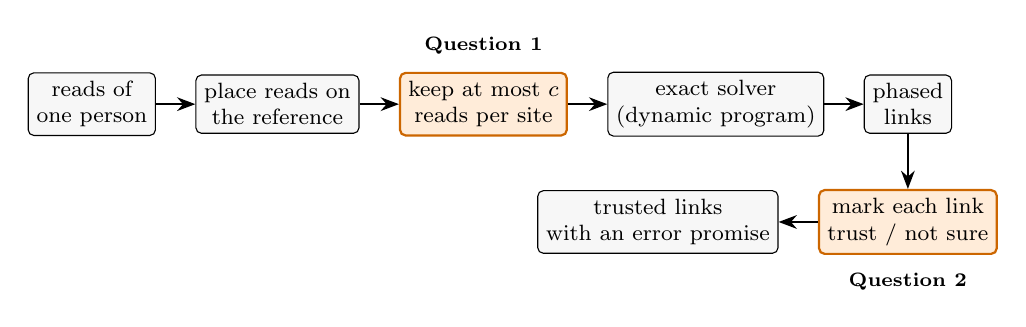
\begin{tikzpicture}[node distance=4mm and 5mm]
  \node[box] (reads) {reads of\\one person};
  \node[box,right=of reads] (align) {place reads on\\the reference};
  \node[hl,right=of align] (sel) {keep at most $c$\\reads per site};
  \node[box,right=of sel] (dp) {exact solver\\(dynamic program)};
  \node[box,right=of dp] (phase) {phased\\links};
  \node[hl,below=7mm of phase] (trust) {mark each link\\trust / not sure};
  \node[box,left=of trust] (out) {trusted links\\with an error promise};
  \draw[arr] (reads)--(align); \draw[arr] (align)--(sel);
  \draw[arr] (sel)--(dp); \draw[arr] (dp)--(phase);
  \draw[arr] (phase)--(trust); \draw[arr] (trust)--(out);
  \node[font=\scriptsize\bfseries,above=1mm of sel] {Question 1};
  \node[font=\scriptsize\bfseries,below=1mm of trust] {Question 2};
\end{tikzpicture}
\caption{Where the two questions sit in a phasing pipeline.}
\label{fig:pipeline}
\end{figure}

Question 1 is about which reads to keep.
WhatsHap~\cite{patterson2015,martin2016} finds the best answer exactly, but
its exact method slows down sharply when many reads overlap. So it first
throws reads away until at most a fixed number (the \emph{cap}) cover each
position, using a quick greedy rule~\cite{fischer2016}. I ask whether a
better choice of reads gives fewer errors (Section~\ref{sec:whatshap}).

Question 2 is about when to trust the answer. I ask whether each phased
link can come with an error promise that still holds on people the method
has never seen (Sections~\ref{sec:promise} to~\ref{sec:rule}). Clinical
guidelines (ACMG/AMP) count \enquote{this variant sits on the other copy from a
known disease variant} as evidence for a recessive disease (code
PM3)~\cite{richards2015}. The standard VCF file has a field, \code{PQ}, for
the chance that a phase is wrong. WhatsHap, HiPhase and LongPhase all leave
it empty.

Min-cost flow and Learn then Test are known methods. This project applies
them to phasing, proves how much data a promise needs, tests every promise
on people not used for tuning, finds why promises break, and measures the
read selector that WhatsHap ships. All data are public, all runs were on the
KCDH server, and every number comes from a run file and a scoring script in
\code{github.com/Nirraaav/phasebudget}. The file
\code{docs/presentation/numbers.tsv} links 74 of the report's main numbers
to the run file and line they come from, and
\code{scripts/check\_report\_numbers.py} checks that each one is still
there. Figure~\ref{fig:glance} lists the
main answers.

\begin{figure}[h]
\centering
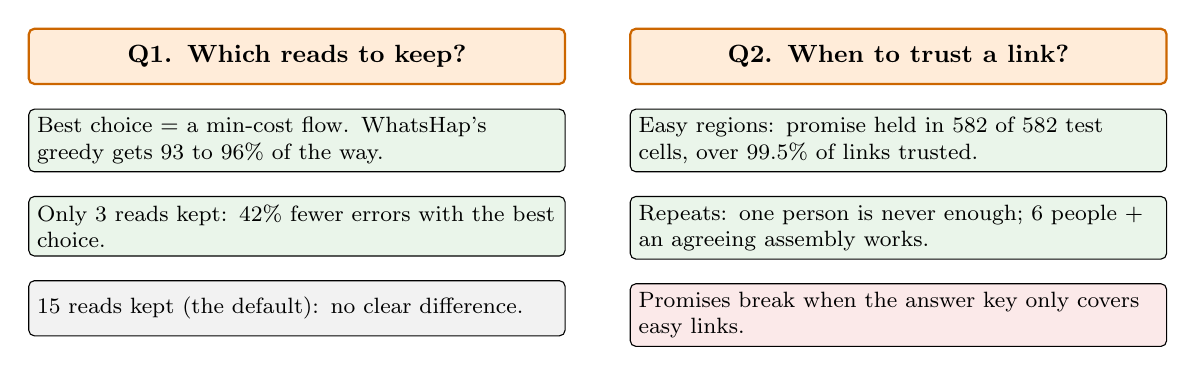
\begin{tikzpicture}[node distance=3mm and 4mm,
  q/.style={box,fill=orange!15,draw=orange!80!black,thick,text width=6.6cm,font=\small\bfseries},
  a/.style={box,text width=6.6cm,align=left,font=\footnotesize}]
  \node[q] (q1) {Q1. Which reads to keep?};
  \node[a,below=of q1,fill=good!10] (a1) {Best choice = a min-cost flow.
    WhatsHap's greedy gets 93 to 96\% of the way.};
  \node[a,below=of a1,fill=good!10] (a2) {Only 3 reads kept: 42\% fewer errors with the best choice.};
  \node[a,below=of a2,fill=gray!10] (a3) {15 reads kept (the default): no clear difference.};
  \node[q,right=8mm of q1] (q2) {Q2. When to trust a link?};
  \node[a,below=of q2,fill=good!10] (b1) {Easy regions: promise held in 582 of 582
    test cells, over 99.5\% of links trusted.};
  \node[a,below=of b1,fill=good!10] (b2) {Repeats: one person is never enough;
    6 people + an agreeing assembly works.};
  \node[a,below=of b2,fill=bad!10] (b3) {Promises break when the answer key
    only covers easy links.};
\end{tikzpicture}
\caption{The project's answers at a glance. Green: what worked; grey: no
effect; red: the main way promises fail.}
\label{fig:glance}
\end{figure}

\paragraph{How to read this report.} Figure~\ref{fig:roadmap} shows the
order of the sections. Readers new to biology should start with
Section~\ref{sec:primer}, which explains DNA, sequencing and reads with no
prior knowledge. Each result in the report is one of three kinds, and the
text says which:
\begin{itemize}
\item \emph{proved}: a mathematical statement that holds for any data;
\item \emph{tested on unseen data}: the method was fixed first and then
  checked, unchanged, on data it had never used, usually new people;
\item \emph{measured on data already seen}: a finding from data that was
  also used to design the method. These results are useful but weaker.
\end{itemize}
Table~\ref{tab:strength} in Section~\ref{sec:summary} sorts every main
result into these three kinds.

\begin{figure}[h]
\centering
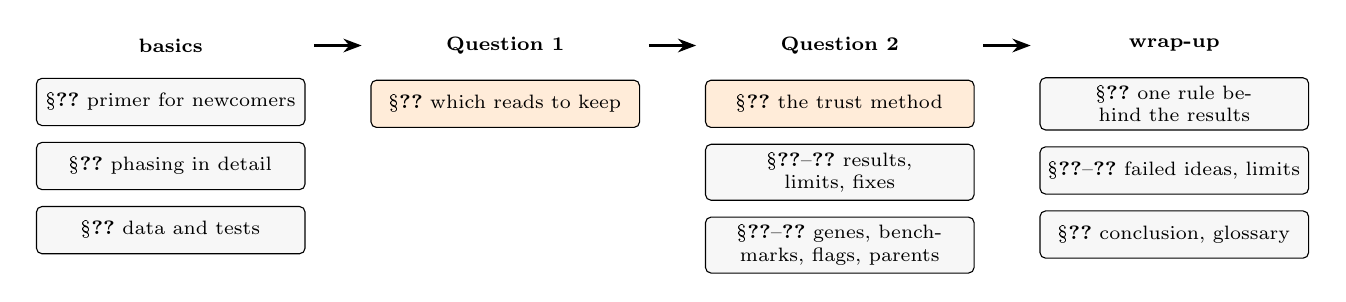
\begin{tikzpicture}[node distance=2mm and 3mm,
  s/.style={box,text width=3.2cm,font=\scriptsize,minimum height=6mm},
  h/.style={font=\scriptsize\bfseries,text width=3.4cm,align=center}]
  \node[h] (h1) {basics};
  \node[s,below=of h1] (b1) {\S\ref{sec:primer} primer for newcomers};
  \node[s,below=of b1] (b2) {\S\ref{sec:bio} phasing in detail};
  \node[s,below=of b2] (b3) {\S\ref{sec:data} data and tests};
  \node[h,right=6mm of h1] (h2) {Question 1};
  \node[s,below=of h2,fill=orange!15] (c1) {\S\ref{sec:whatshap} which reads to keep};
  \node[h,right=6mm of h2] (h3) {Question 2};
  \node[s,below=of h3,fill=orange!15] (d1) {\S\ref{sec:promise} the trust method};
  \node[s,below=of d1] (d2) {\S\ref{sec:held}--\ref{sec:keys} results, limits, fixes};
  \node[s,below=of d2] (d3) {\S\ref{sec:genes}--\ref{sec:na12878} genes, benchmarks, flags, parents};
  \node[h,right=6mm of h3] (h4) {wrap-up};
  \node[s,below=of h4] (e1) {\S\ref{sec:rule} one rule behind the results};
  \node[s,below=of e1] (e2) {\S\ref{sec:honest}--\ref{sec:limits} failed ideas, limits};
  \node[s,below=of e2] (e3) {\S\ref{sec:summary} conclusion, glossary};
  \draw[arr] (h1) -- (h2); \draw[arr] (h2) -- (h3); \draw[arr] (h3) -- (h4);
\end{tikzpicture}
\caption{A map of the report.}
\label{fig:roadmap}
\end{figure}

%=====================================================================
\section{A primer for readers new to biology}\label{sec:primer}
%=====================================================================

This section assumes no biology. It explains the four ideas the rest of the
report needs: DNA, the two copies, reading DNA, and why long reads help.
Section~\ref{sec:bio} then goes into the details of phasing.

\subsection{DNA is a long text}

Every cell of the body holds the same instruction manual, the
\emph{genome}. It is written in DNA, a molecule that can be read as a text
over four letters: \dna{A}, \dna{C}, \dna{G} and \dna{T}. The human genome
has about 3 billion letters. It is not one long string; it is split into 23
pieces called \emph{chromosomes}, which work like the volumes of an
encyclopedia (Figure~\ref{fig:cell}). A \emph{gene} is a passage in one
volume that tells the cell how to build one protein.

\begin{figure}[h]
\centering
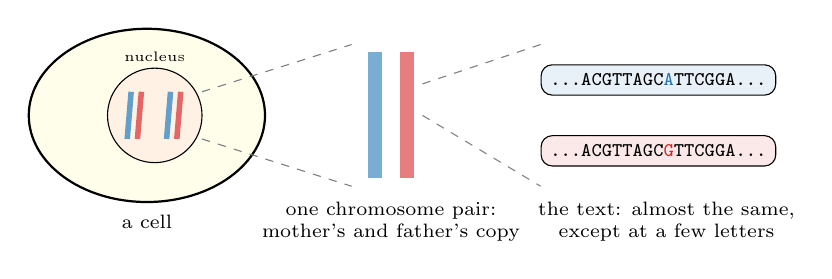
\begin{tikzpicture}[font=\scriptsize]
  % cell
  \draw[thick,fill=yellow!8] (0,0) ellipse (1.5 and 1.1);
  \draw[fill=orange!10] (0.1,0) circle (0.6);
  \node at (0,-1.35) {a cell};
  \foreach \x/\c in {-0.25/hapA,-0.12/hapB,0.25/hapA,0.38/hapB}
    \draw[line width=2pt,\c!70] (\x,-0.3) -- (\x+0.05,0.3);
  \node[font=\tiny] at (0.1,0.75) {nucleus};
  % zoom to chromosome pair
  \draw[gray,dashed] (0.7,0.3) -- (2.6,0.9); \draw[gray,dashed] (0.7,-0.3) -- (2.6,-0.9);
  \draw[line width=5pt,hapA!60,rounded corners] (2.9,-0.8) -- (2.9,0.8);
  \draw[line width=5pt,hapB!60,rounded corners] (3.3,-0.8) -- (3.3,0.8);
  \node[align=center] at (3.1,-1.35) {one chromosome pair:\\mother's and father's copy};
  % zoom to letters
  \draw[gray,dashed] (3.5,0.4) -- (5.0,0.9); \draw[gray,dashed] (3.5,0.0) -- (5.0,-0.9);
  \node[draw,rounded corners,fill=hapA!10,anchor=west,font=\ttfamily\scriptsize] at (5.0,0.45)
     {...ACGTTAGC\textcolor{hapA}{\textbf{A}}TTCGGA...};
  \node[draw,rounded corners,fill=hapB!10,anchor=west,font=\ttfamily\scriptsize] at (5.0,-0.45)
     {...ACGTTAGC\textcolor{hapB}{\textbf{G}}TTCGGA...};
  \node[align=center] at (6.6,-1.35) {the text: almost the same,\\except at a few letters};
\end{tikzpicture}
\caption{From a cell to the letters of DNA. Each chromosome comes in two
copies, one from each parent. The copies differ at a few positions, like the
bold letter here.}
\label{fig:cell}
\end{figure}

\paragraph{Two copies of every volume.} Each person has two copies of every
chromosome: one set of 23 from the mother and one set of 23 from the father.
The two copies of a chromosome are almost identical, but they differ at
about one letter in every 1{,}000 to 1{,}500. These differences are what
make people different from each other, and some of them cause disease.

\subsection{Reading DNA: sequencing and reads}

No machine can read a whole chromosome from end to end. A
\emph{sequencer} instead reads millions of random pieces of DNA, called
\emph{reads}. A computer then finds where each read belongs by matching it
against a standard human genome, the \emph{reference genome}, much as one
would place the pieces of a jigsaw by looking at the picture on the box
(Figure~\ref{fig:sequencing}). Where a read has a different letter from the
reference, the person may carry a \emph{variant} there.

\begin{figure}[h]
\centering
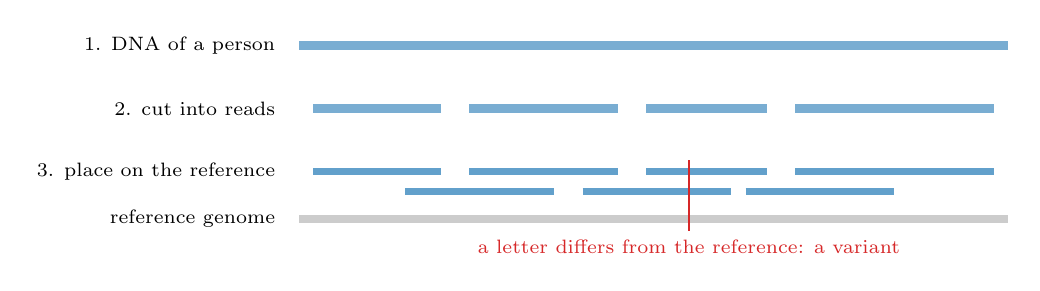
\begin{tikzpicture}[font=\scriptsize,x=0.9cm]
  \node[anchor=east] at (-0.2,2.2) {1. DNA of a person};
  \draw[line width=3pt,hapA!60] (0,2.2) -- (10,2.2);
  \node[anchor=east] at (-0.2,1.4) {2. cut into reads};
  \foreach \a/\b in {0.2/2.0,2.4/4.5,4.9/6.6,7.0/9.8}
    \draw[line width=3pt,hapA!60] (\a,1.4) -- (\b,1.4);
  \node[anchor=east] at (-0.2,0.6) {3. place on the reference};
  \draw[line width=3pt,gray!40] (0,0) -- (10,0);
  \node[anchor=east] at (-0.2,0) {reference genome};
  \foreach \a/\b/\y in {0.2/2.0/0.6,1.5/3.6/0.35,2.4/4.5/0.6,4.0/6.1/0.35,4.9/6.6/0.6,6.3/8.4/0.35,7.0/9.8/0.6}
    \draw[line width=2.5pt,keep!70] (\a,\y) -- (\b,\y);
  \draw[bad,thick] (5.5,-0.15) -- (5.5,0.75);
  \node[bad,anchor=north] at (5.5,-0.15) {a letter differs from the reference: a variant};
\end{tikzpicture}
\caption{Sequencing in three steps: the machine reads random pieces, and a
computer places each piece where it matches the reference genome. Several
reads cover each position.}
\label{fig:sequencing}
\end{figure}

\paragraph{Coverage.} Because the pieces are random, each position is
covered by several reads. The average number is the \emph{coverage}, or
depth: at 30$\times$, each letter is read about 30 times. Reads also contain
reading mistakes, so a single read can be wrong; many reads together are
reliable.

\subsection{Why long reads matter here}

Older machines produce \emph{short reads} of about 150 letters. Since
variants are about 1{,}000 letters apart, a short read usually contains at
most one variant, and so it cannot tell which variants sit on the same copy.
Newer \emph{long-read} machines (PacBio HiFi and Oxford Nanopore) produce
reads of 10{,}000 letters or more. One long read covers several variants
at once, and because each read comes from one copy, it shows which letters
go together (Figure~\ref{fig:longreads}). This project uses long reads only.

\begin{figure}[h]
\centering
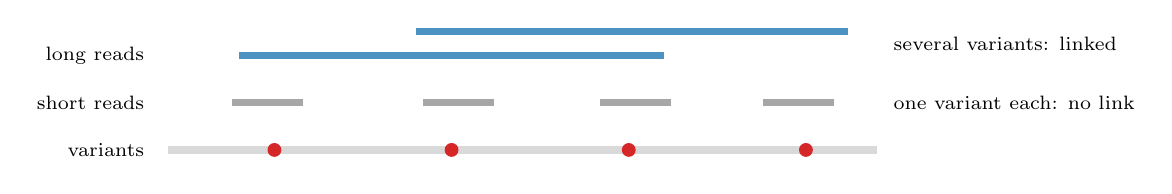
\begin{tikzpicture}[font=\scriptsize,x=0.9cm]
  \draw[line width=3pt,gray!30] (0,0) -- (10,0);
  \foreach \x in {1.5,4,6.5,9} {\fill[bad] (\x,0) circle (2.5pt);}
  \node[anchor=east] at (-0.2,0) {variants};
  \node[anchor=east] at (-0.2,0.6) {short reads};
  \foreach \a in {0.9,3.6,6.1,8.4} \draw[line width=2.5pt,gray!70] (\a,0.6) -- (\a+1.0,0.6);
  \node[anchor=west] at (10.1,0.6) {one variant each: no link};
  \node[anchor=east] at (-0.2,1.2) {long reads};
  \draw[line width=2.5pt,keep!80] (1.0,1.2) -- (7.0,1.2);
  \draw[line width=2.5pt,keep!80] (3.5,1.5) -- (9.6,1.5);
  \node[anchor=west] at (10.1,1.35) {several variants: linked};
\end{tikzpicture}
\caption{A short read rarely covers two variants. A long read covers several
and shows which of their letters sit on the same copy.}
\label{fig:longreads}
\end{figure}

\subsection{Where computing comes in}

Turning millions of noisy reads into the two copies of each chromosome is a
computing problem with two parts, and they are the two questions of this
report:
\begin{itemize}
\item an \emph{optimisation} problem: the exact solver can only handle a few
  reads at each position, so some must be dropped, and the question is
  which (Question 1, Section~\ref{sec:whatshap});
\item a \emph{statistics} problem: some answers will be wrong, and the
  question is how to say which answers can be trusted, with an error rate
  that holds on new people (Question 2, Sections~\ref{sec:promise}
  to~\ref{sec:rule}).
\end{itemize}

\subsection{Phasing and the other omics}

The other layers studied in this course, such as RNA and DNA methylation,
are also measured per copy, and a phased genome is what lets them be split
by copy (Figure~\ref{fig:omics}).
\begin{itemize}
\item \emph{RNA.} A gene's two copies can be read into RNA at different
  rates (allele-specific expression). Reads of RNA carry the same variant
  letters, so a phase tells which copy each RNA molecule came from.
\item \emph{Methylation.} Chemical marks on DNA switch genes off, sometimes
  only on the copy from one parent (imprinting). Nanopore reads record these
  marks, and a phase groups them by copy. Section~\ref{sec:honest} reports
  one attempt to use them to tell which copy came from which parent.
\item \emph{Diagnosis.} Two harmful variants in one gene mean a healthy
  carrier if they are on the same copy and a sick child if not
  (Section~\ref{sec:bio}).
\end{itemize}

\begin{figure}[h]
\centering
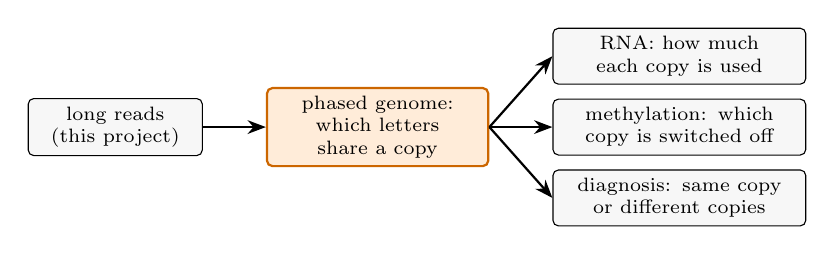
\begin{tikzpicture}[node distance=4mm and 8mm,
  o/.style={box,text width=3.0cm,font=\scriptsize}]
  \node[hl,text width=2.6cm,font=\scriptsize] (p) {phased genome:\\which letters share a copy};
  \node[o,right=of p,yshift=9mm] (r) {RNA: how much each copy is used};
  \node[o,right=of p] (m) {methylation: which copy is switched off};
  \node[o,right=of p,yshift=-9mm] (d) {diagnosis: same copy or different copies};
  \node[box,left=of p,text width=2.0cm,font=\scriptsize] (l) {long reads\\(this project)};
  \draw[arr] (l) -- (p);
  \draw[arr] (p.east) -- (r.west); \draw[arr] (p.east) -- (m.west); \draw[arr] (p.east) -- (d.west);
\end{tikzpicture}
\caption{A phased genome is the base on which other layers can be split by
copy. An error in the phase becomes an error in every layer built on it,
which is why Question 2 asks for a stated error rate.}
\label{fig:omics}
\end{figure}

%=====================================================================
\section{Background}\label{sec:bio}
%=====================================================================

\subsection{Two copies, heterozygous sites, links}

The two copies of a chromosome differ at about one position in 1{,}000 to
1{,}500 (Section~\ref{sec:primer}), which gives a few million positions per
person. These positions are called \emph{heterozygous sites}. At each site I
write \dna{0} for the letter in the reference genome and \dna{1} for the
other letter.

A standard DNA test reports both letters at each site, but not which letters
share a copy. Think of it with words instead of DNA:

\begin{center}
\small
\begin{tabular}{@{}ll@{}}
mother's copy & \dna{THE CAT SAT ON THE MAT}\\
father's copy & \dna{THE CAT SA\textcolor{hapB}{W} ON THE \textcolor{hapB}{H}AT}\\
\end{tabular}
\end{center}

The test sees \enquote{\dna{T} or \dna{W}} and \enquote{\dna{M} or \dna{H}}, but it
cannot tell \{\dna{SAT\dots MAT}, \dna{SAW\dots HAT}\} apart from
\{\dna{SAT\dots HAT}, \dna{SAW\dots MAT}\}. Deciding which is right is
\emph{phasing}. With $n$ sites there are $2^{n-1}$ possible answers
(swapping the two copies gives the same answer, hence $n-1$).

For two sites the answer is a single yes/no: \emph{cis} if the two \dna{1}s
are on the same copy, \emph{trans} if they are on different copies. A cis or
trans answer between two neighbouring sites is called a \emph{link}
(Figure~\ref{fig:links}). A chromosome with $n$ phased sites has $n-1$
links. Accuracy is measured by counting wrong links (\enquote{switch errors}),
usually per 10{,}000 links.

\begin{figure}[h]
\centering
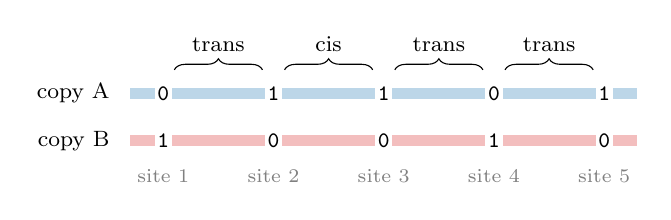
\begin{tikzpicture}[x=1.4cm,font=\footnotesize]
  \draw[line width=4pt,hapA!30] (-0.3,0.6) -- (4.3,0.6);
  \draw[line width=4pt,hapB!30] (-0.3,0) -- (4.3,0);
  \node[anchor=east] at (-0.4,0.6) {copy A}; \node[anchor=east] at (-0.4,0) {copy B};
  \foreach \i/\a/\b in {0/0/1,1/1/0,2/1/0,3/0/1,4/1/0} {
    \node[fill=white,inner sep=1pt] at (\i,0.6) {\dna{\a}};
    \node[fill=white,inner sep=1pt] at (\i,0) {\dna{\b}};
    \node[gray,font=\scriptsize] at (\i,-0.45) {site \the\numexpr\i+1\relax};}
  \foreach \i/\r in {0/trans,1/cis,2/trans,3/trans} {
    \draw[decorate,decoration={brace,amplitude=4pt}] (\i+0.1,0.9) -- (\i+0.9,0.9)
      node[midway,above=3pt] {\r};}
\end{tikzpicture}
\caption{Five sites, four links. Each link says whether the \dna{1}s of two
neighbouring sites sit on the same copy (cis) or on different copies
(trans).}
\label{fig:links}
\end{figure}

\begin{figure}[h]
\centering
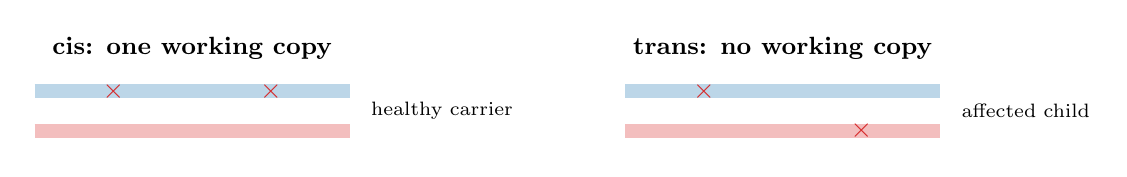
\begin{tikzpicture}[x=0.5cm,y=0.5cm]
  \node[font=\small\bfseries] at (4,4.1) {cis: one working copy};
  \draw[line width=5pt,hapA!30] (0,3) -- (8,3);
  \draw[line width=5pt,hapB!30] (0,2) -- (8,2);
  \node[bad,font=\bfseries] at (2,3) {$\times$}; \node[bad,font=\bfseries] at (6,3) {$\times$};
  \node[anchor=west,font=\scriptsize] at (8.3,2.5) {healthy carrier};
  \begin{scope}[xshift=7.5cm]
  \node[font=\small\bfseries] at (4,4.1) {trans: no working copy};
  \draw[line width=5pt,hapA!30] (0,3) -- (8,3);
  \draw[line width=5pt,hapB!30] (0,2) -- (8,2);
  \node[bad,font=\bfseries] at (2,3) {$\times$}; \node[bad,font=\bfseries] at (6,2) {$\times$};
  \node[anchor=west,font=\scriptsize] at (8.3,2.5) {affected child};
  \end{scope}
\end{tikzpicture}
\caption{Two damaging variants ($\times$) in one gene, on the two copies of a chromosome.}
\label{fig:cistrans}
\end{figure}

\paragraph{Medical use.} Take a gene such as CFTR (cystic fibrosis). If
two damaging changes sit on the same copy (cis), the other copy still works:
the person is a healthy carrier. If they sit on different copies (trans), no
working copy is left: the child is affected (Figure~\ref{fig:cistrans}). A
genome has about 3 million links, so even 999 right out of 1{,}000 leaves
about 3{,}000 wrong. An average accuracy does not tell a doctor whether the
one link they care about is among them. A doctor needs to know which answers
to rely on.

\subsection{Reads, and phasing as a vote}

Phasing works like a vote. Every read that covers two sites votes for cis
or for trans. Reads contain reading mistakes, so some votes are wrong
(Figure~\ref{fig:votes}).

\begin{figure}[h]
\centering
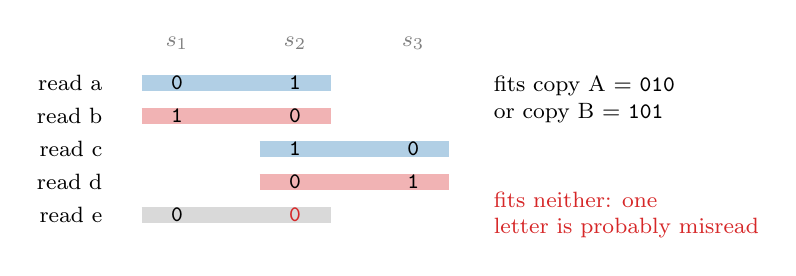
\begin{tikzpicture}[x=1.5cm,y=0.42cm,font=\footnotesize]
  \foreach \i in {1,2,3} \node[gray] at (\i,5.2) {$s_\i$};
  \foreach \y/\n in {4/a,3/b,2/c,1/d,0/e}
    \node[anchor=east] at (0.45,\y) {read \n};
  \draw[line width=6pt,hapA!35] (0.7,4) -- (2.3,4);
  \draw[line width=6pt,hapB!35] (0.7,3) -- (2.3,3);
  \draw[line width=6pt,hapA!35] (1.7,2) -- (3.3,2);
  \draw[line width=6pt,hapB!35] (1.7,1) -- (3.3,1);
  \draw[line width=6pt,gray!30] (0.7,0) -- (2.3,0);
  \node at (1,4) {\dna{0}}; \node at (2,4) {\dna{1}};
  \node at (1,3) {\dna{1}}; \node at (2,3) {\dna{0}};
  \node at (2,2) {\dna{1}}; \node at (3,2) {\dna{0}};
  \node at (2,1) {\dna{0}}; \node at (3,1) {\dna{1}};
  \node at (1,0) {\dna{0}}; \node[bad,font=\footnotesize\bfseries] at (2,0) {\dna{0}};
  \node[anchor=west,align=left] at (3.6,3.5) {fits copy A = \dna{010}\\or copy B = \dna{101}};
  \node[anchor=west,bad,align=left] at (3.6,0) {fits neither: one\\letter is probably misread};
\end{tikzpicture}
\caption{Five reads over three sites. Blue reads fit copy A, red reads fit
copy B, and read e disagrees with both by one letter.}
\label{fig:votes}
\end{figure}

To find the best answer, try each possible pair of copies. Match each read
to the copy it fits best and count the letters that would have to change.
The pair needing the fewest changes wins:

\begin{center}
\small
\begin{tabular}{@{}lccc@{}}
\toprule
read & $s_1$ & $s_2$ & $s_3$\\
\midrule
a & 0 & 1 & \\
b & 1 & 0 & \\
c &   & 1 & 0\\
d &   & 0 & 1\\
e & 0 & 0 & \\
\bottomrule
\end{tabular}
\qquad
\begin{tabular}{@{}lr@{}}
\toprule
copies A / B & changes\\
\midrule
\dna{000} / \dna{111} & 4\\
\dna{001} / \dna{110} & 2\\
\dna{010} / \dna{101} & 1\\
\dna{011} / \dna{100} & 3\\
\bottomrule
\end{tabular}
\qquad
\begin{minipage}{6.2cm}\small
Best: \dna{010}/\dna{101}. Reads a, c fit A; b, d fit B; read e
(\dna{00}) is one letter off both copies, so it probably has a mistake.
\end{minipage}
\end{center}

Picking the pair of copies with the fewest changes is called \emph{minimum
error correction} (MEC). In practice each change is weighted by how sure the
machine was about that letter (its \emph{base quality}): changing a letter
the machine was unsure about costs little. This is weighted MEC.

\subsection{Why the exact solver drops reads}

WhatsHap solves weighted MEC exactly with a \emph{dynamic program}: it walks
along the sites one by one, and at each site it keeps track of every way to
split that site's reads between copy A and copy B. With $c$ reads there are
$2^c$ splits, so the work doubles with every extra read
(Figure~\ref{fig:blowup}). That is why WhatsHap keeps at most 15 reads per
site (the \emph{cap}), picked by a quick greedy rule, and drops the rest.
HiPhase~\cite{holt2024} and LongPhase~\cite{lin2022} keep all reads instead,
but their solvers are not guaranteed to find the best answer.

\begin{figure}[h]
\centering
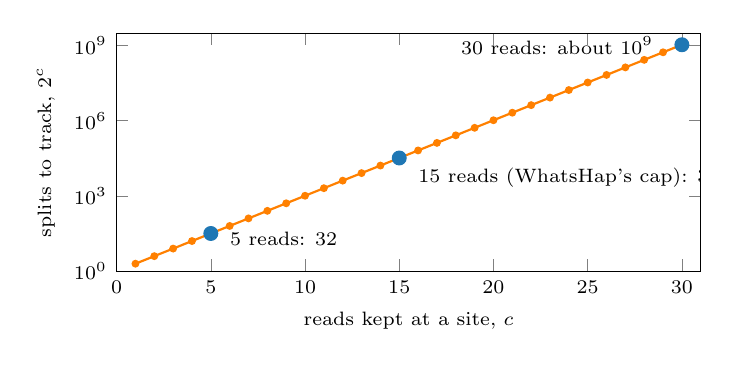
\begin{tikzpicture}
\begin{axis}[width=9cm,height=4.6cm,ymode=log,xmin=0,xmax=31,ymin=1,ymax=3e9,
  xlabel={reads kept at a site, $c$},ylabel={splits to track, $2^c$},
  tick label style={font=\scriptsize},label style={font=\scriptsize},
  ytick={1,1e3,1e6,1e9}]
\addplot[thick,orange,domain=1:30,samples=30,mark=*,mark size=1pt] {2^x};
\addplot[only marks,mark=*,mark size=2.5pt,keep] coordinates {(5,32) (15,32768) (30,1073741824)};
\node[font=\scriptsize,anchor=west] at (axis cs:5.5,20) {5 reads: 32};
\node[font=\scriptsize,anchor=north west] at (axis cs:15.5,32768) {15 reads (WhatsHap's cap): 32{,}768};
\node[font=\scriptsize,anchor=east] at (axis cs:29,1e9) {30 reads: about $10^9$};
\end{axis}
\end{tikzpicture}
\caption{The exact solver's work doubles with every extra read, so reads
must be dropped.}
\label{fig:blowup}
\end{figure}

\subsection{What already exists}

\begin{itemize}
\item Picking the best reads under a per-site cap is a known scheduling
  problem, solved exactly by min-cost flow~\cite{arkin1987,carlisle1995}.
  Fischer and
  Marschall~\cite{fischer2016} planned to compare their greedy rule with
  the flow method of M\"akinen et al.~\cite{makinen2015}, but I found no
  report of that comparison. (If gaps inside a read did not count towards
  the cap, the problem would become much harder:
  APX-hard~\cite{bareyehuda2006}.)
\item The true pair of copies can need more changes than a wrong
  pair~\cite{duitama2012,majidian2020}, so I report both the MEC cost and
  the accuracy.
\item HapCUT2~\cite{hapcut2} drops sites whose
  estimated probability is below 0.8, but I found no check that these
  probabilities are right. PhaseQuality~\cite{damaraju2026} sorts pairs into
  confidence tiers, which are not probabilities. Phasing from population
  data gives a probability per site~\cite{shapeit5}; phasing from reads has
  nothing like it.
\item Methods that let a predictor say
  \enquote{not sure}~\cite{geifman2017}, and Learn then Test~\cite{ltt2025}, pick
  a threshold with a stated error rate. Doing this separately per category
  goes back to Vovk~\cite{vovk2012}; here the categories are region types.
\end{itemize}

\subsection{Words used}

A few words have a fixed meaning in this report. An \emph{answer key} is a
phase believed to be correct, used to score phasers (other papers call it a
truth set). A \emph{stretch} is a 100\,kb window of a chromosome. Each link
belongs to one of six \emph{region types}, which group the genome by how hard
it is to phase (Section~\ref{sec:regions}). When the method says \emph{not
sure} about a link, it declines to vouch for it. Test results are reported
in \emph{cells}: a cell is one combination of test person, coverage, phaser,
error target $\beta$ and region type. A cell \emph{breaks} when it has
significantly more bad stretches than the promise allows.

%=====================================================================
\section{Data}\label{sec:data}
%=====================================================================

\paragraph{People.} The project used 48 people whose data are public: the
Genome in a Bottle (GIAB) reference people
HG002 and HG005; HG001 (also called NA12878) and six relatives from a
four-generation family (the Platinum Pedigree, family CEPH~1463); and 39
people from the Human Pangenome project (HPRC) of African, admixed American
and East Asian ancestry. Reads are Nanopore and PacBio HiFi at 10$\times$ to
30$\times$.


\paragraph{Answer keys.} To count errors we need to know the true phase. Each
person's phase is scored against an \emph{answer key}, a phase believed to
be correct:

\begin{center}
\small
\begin{tabular}{@{}p{4.2cm}p{11cm}@{}}
\toprule
people & answer key\\
\midrule
HG002 & near-perfect assembly of both copies (Q100, GIAB v5.0q~\cite{hansen2026})\\
HG001 and six relatives & the four-generation family (Platinum Pedigree~\cite{kronenberg2025})\\
HG005 & what the parents passed down (a \enquote{trio})\\
39 HPRC people & the person's assembly, checked against the parents\\
\bottomrule
\end{tabular}
\end{center}

\paragraph{Experiments.} The work has two parts. First, six runs on read
selection, five in my own phasing library and one inside
\code{whatshap phase}:

\begin{itemize}
\item a pilot on HG002 HiFi chromosome 20, with 8 pipelines and 4 caps;
\item HG002 HiFi on 21 chromosomes, at 4 depths, with 10 rules;
\item HG002 Nanopore with the same design, plus a vote-model prediction;
\item HG005 HiFi with the same design, as a second person;
\item HG002 with both parents, in WhatsHap's family mode;
\item \code{whatshap phase} itself on HG002 HiFi, greedy against optimal
  (the \enquote{HiFi tool run}).
\end{itemize}

Then come twelve tests, one more inside \code{whatshap phase} and eleven of
the trust method. In every test the method is tuned on some people and then
checked, unchanged, on other people.

\begin{itemize}
\item Test 1 puts the optimal read choice inside \code{whatshap phase}, on HG002 Nanopore.
\item Test 2 uses one cutoff for the whole genome, on HG001 and HG002.
\item Test 3 uses one cutoff per region type, on 6 relatives and HG005.
\item Test 4 repeats Test 3 with a newer basecaller, on HG001.
\item Test 5 repeats it on other ancestries, on 39 HPRC people.
\item Test 6 pools cutoffs from 21 people, on 5 family members and 19 HPRC people.
\item Test 7 trusts only links an assembly agrees with, on NA12877 and HG005.
\item Test 8 makes gene-level calls with the assembly rule, on NA12877 and HG005.
\item Test 9 uses labels from parents only, on HG005.
\item Test 10 counts errors outside the benchmark region, on HG005.
\item Test 11 checks the answer-key effect on 19 new HPRC people.
\item Test 12 checks five predictions on a new person, NA12878.
\end{itemize}

%=====================================================================
\section{Which reads to keep}\label{sec:whatshap}
%=====================================================================

\subsection{The selection problem}

In words: give each read a value (how much it tells us), and keep the most
valuable set of reads such that no site is covered by more than $c$ kept
reads. In symbols, number the sites $1,\dots,n$. Read $r$ covers the
consecutive sites $a_r,\dots,b_r$ and has weight $w_r$, the sum of its base
qualities. A site inside a read's span that the read did not call (a gap)
still counts towards the cap there. Selection is
\[
\max \sum_r w_r x_r \quad\text{s.t.}\quad \sum_{r:\,a_r\le j\le b_r} x_r\le c
\ \ \text{for every site } j,\qquad x_r\in\{0,1\}.
\]

\paragraph{Greedy can miss the best choice.} A greedy rule takes the
best-looking read first, and that can block a better combination. Example:
four sites, cap 2, and a read's weight is the number of sites it covers
(Figure~\ref{fig:greedy}). Greedy takes R1 (weight 4), then R4 (weight 2).
Now sites 2 and 3 already hold 2 reads each, so R2 and R3 no longer fit:
total 6. Keeping R1, R2 and R3 instead gives 8.

\begin{figure}[h]
\centering
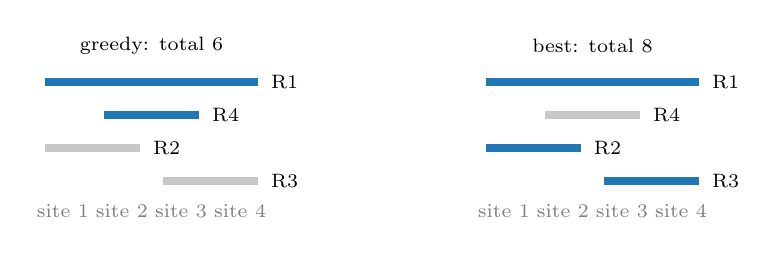
\begin{tikzpicture}[x=0.75cm,y=0.42cm,font=\scriptsize]
  \node at (2.5,4.1) {greedy: total 6};
  \foreach \i in {1,...,4} \node[gray] at (\i,-0.9) {site \i};
  \draw[line width=3pt,keep] (0.7,3) -- (4.3,3) node[right,black] {R1};
  \draw[line width=3pt,keep] (1.7,2) -- (3.3,2) node[right,black] {R4};
  \draw[line width=3pt,drop] (0.7,1) -- (2.3,1) node[right,black] {R2};
  \draw[line width=3pt,drop] (2.7,0) -- (4.3,0) node[right,black] {R3};
  \begin{scope}[xshift=5.6cm]
  \node at (2.5,4.1) {best: total 8};
  \foreach \i in {1,...,4} \node[gray] at (\i,-0.9) {site \i};
  \draw[line width=3pt,keep] (0.7,3) -- (4.3,3) node[right,black] {R1};
  \draw[line width=3pt,drop] (1.7,2) -- (3.3,2) node[right,black] {R4};
  \draw[line width=3pt,keep] (0.7,1) -- (2.3,1) node[right,black] {R2};
  \draw[line width=3pt,keep] (2.7,0) -- (4.3,0) node[right,black] {R3};
  \end{scope}
\end{tikzpicture}
\caption{Kept reads in blue, dropped reads in grey.}
\label{fig:greedy}
\end{figure}

\subsection{The best choice is a min-cost flow}

Each read covers an unbroken run of sites, like a hotel booking for a run of
consecutive nights in a hotel with $c$ rooms. Problems of this shape
(interval scheduling with capacity $c$~\cite{arkin1987,carlisle1995}) can be
solved exactly and quickly as a \emph{min-cost flow}. Build a network as in
Figure~\ref{fig:flow}:

\begin{itemize}
\item nodes $v_0,\dots,v_n$; a \emph{chain arc} $v_{j-1}\to v_j$ for each
  site $j$, capacity $c$, cost 0;
\item a \emph{read arc} $v_{a_r-1}\to v_{b_r}$ for each read, capacity 1,
  cost $-w_r$;
\item send $c$ units from $v_0$ to $v_n$.
\end{itemize}

\begin{figure}[h]
\centering
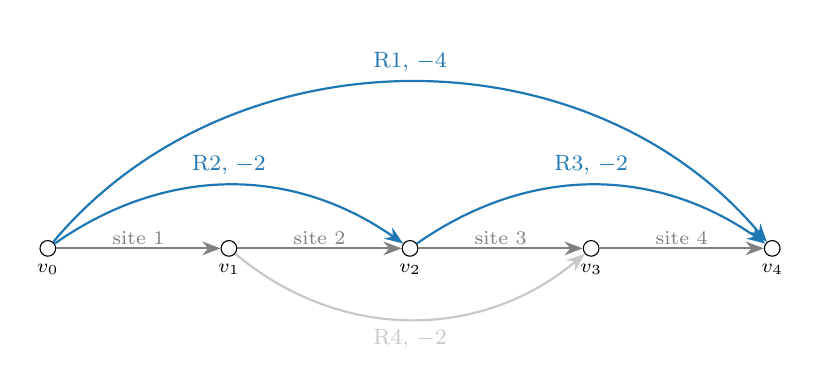
\begin{tikzpicture}[x=2.3cm,y=0.9cm,font=\footnotesize,
   n/.style={circle,draw,inner sep=2pt,fill=white}]
  \foreach \i in {0,...,4} \node[n] (s\i) at (\i,0) {};
  \foreach \i in {0,...,4} \node[below=2pt,font=\scriptsize] at (s\i) {$v_\i$};
  \foreach \i/\j in {0/1,1/2,2/3,3/4}
    \draw[-{Stealth},thick,gray] (s\i) -- node[above,font=\scriptsize,fill=white,inner sep=1pt] {site \j} (s\j);
  \draw[-{Stealth},keep,thick] (s0) to[bend left=50] node[above] {R1, $-4$} (s4);
  \draw[-{Stealth},keep,thick] (s0) to[bend left=35] node[above] {R2, $-2$} (s2);
  \draw[-{Stealth},keep,thick] (s2) to[bend left=35] node[above] {R3, $-2$} (s4);
  \draw[-{Stealth},drop,thick] (s1) to[bend right=40] node[below] {R4, $-2$} (s3);
\end{tikzpicture}
\caption{The flow network for Figure~\ref{fig:greedy}. Grey chain arcs have capacity $c$ and cost 0; each read arc has capacity 1 and cost minus its weight. Blue arcs carry flow in the optimum.}
\label{fig:flow}
\end{figure}

\emph{Why it works.} Picture $c$ cars driving from $v_0$ to $v_n$. At each
site a car either drives along the chain (no read) or rides inside a read
arc that covers the site. Arcs only go forward, so every car passes every
site exactly once, and at most $c$ kept reads can cover any site. In the
other direction, every allowed choice of reads can be written as such a
flow (spare cars use the chain). The cost is minus the total weight, so the
cheapest flow is the heaviest choice of reads. Because all capacities are
whole numbers, the solver returns a whole-number answer: each read is either
kept or not.

\begin{lstlisting}
def select_optimal(reads, n_sites, cap):        # reads: (id, start, end, weight)
    flow = MinCostFlow(n_nodes=n_sites + 1)
    for j in range(n_sites):                     # chain arc = site j
        flow.add_edge(j, j + 1, capacity=cap, cost=0)
    arc = {r: flow.add_edge(s, e, capacity=1, cost=-w) for r, s, e, w in reads}
    flow.run(source=0, sink=n_sites, units=cap)  # successive shortest paths
    return {r for r, a in arc.items() if flow.carries(a)}
\end{lstlisting}

On 250 random small cases it matched brute force (trying every subset).
The library's four phasing solvers (brute force, a dynamic program in Python
and in C++, an integer program) also agree on the best cost wherever all of
them can run. I compare costs and not phases, because two different phases
can tie for best.

\subsection{The rule WhatsHap ships}

The published rule~\cite{fischer2016} gives each read a score (sites read
minus gaps inside it), breaks ties by the read's lowest base quality, and
takes reads in score order. After each pick it lowers the scores of the
reads still waiting. In the WhatsHap 2.8 code (\code{readselect.pyx}) this
update counts the \emph{opposite} set of sites:

\begin{lstlisting}
# new = sites the read just taken covered for the first time
drop_paper   = sum(1 for s in waiting.sites if s in new)      # published rule
drop_shipped = sum(1 for s in waiting.sites if s not in new)  # WhatsHap 2.8
\end{lstlisting}

There are three smaller differences. Scores change in place inside a
binary heap, so tied reads come out in heap order. A second \enquote{bridging}
pass throws away a read that would break the cap before checking whether it
would join two blocks. Gaps are counted only over sites that some read
covers. In outline:

\begin{lstlisting}
def whatshap_select(reads, cap):
    selected, undecided = set(), set(reads)
    while undecided:
        heap = MaxHeap((score(r), r) for r in undecided)
        covered, this_round, too_full = set(), set(), set()
        while heap:
            r = heap.pop()
            new = [s for s in r.sites if s not in covered]
            if any(count[s] >= cap for s in r.span):
                too_full.add(r)                      # would break the cap
            elif new:
                take(r); this_round.add(r); covered.update(new)
                for q in waiting_reads_touching(new):
                    heap.lower_first_score(q, drop_shipped(q, new))
        selected |= this_round
        undecided -= this_round | too_full
        bridge(undecided)          # add reads that join two blocks, if they fit
    return selected
\end{lstlisting}

I copied the shipped code line by line into Python and checked that my
copy picks the same reads as WhatsHap 2.8 on the same inputs:

\begin{center}
\small
\begin{tabular}{@{}lrr@{}}
\toprule
inputs & my port = WhatsHap & published rule = WhatsHap\\
\midrule
300 small random inputs $\times$ 5 caps & 1{,}500 of 1{,}500 & 178 of 1{,}500\\
36 chromosome-scale inputs & 36 of 36 & not run\\
\bottomrule
\end{tabular}
\end{center}

The last 4 small cases needed one more detail. WhatsHap keeps sites in a
C++ \code{unordered\_set}, and the order in which that set lists its items
(set by its bucket count: 13, 29, 59, 127, \dots) decides which tied read
goes first. My copy imitates that order too.

\paragraph{How far from the best?} At the default cap 15, the shipped greedy
keeps 93 to 96 per cent of the best possible weight (Figure~\ref{fig:gap}),
so it loses 4 to 7 per cent. Picking reads at random keeps 90.5 per cent. To
see whether the lost weight costs accuracy, I compared the two choices in
three steps (Figure~\ref{fig:steps}).

\begin{figure}[h]
\centering
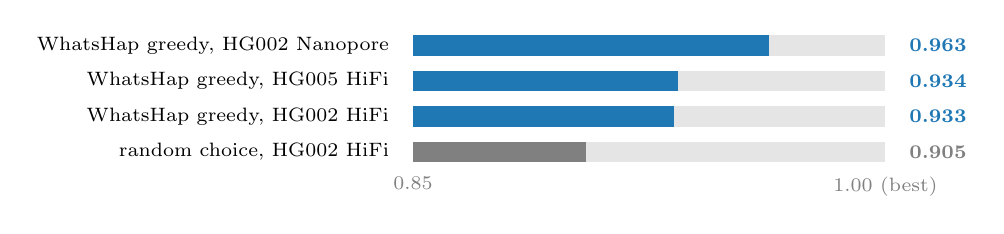
\begin{tikzpicture}[x=6cm]
  \failbar{0}{WhatsHap greedy, HG002 Nanopore}{0.753}{0.963}{keep}
  \failbar{-0.45}{WhatsHap greedy, HG005 HiFi}{0.560}{0.934}{keep}
  \failbar{-0.90}{WhatsHap greedy, HG002 HiFi}{0.553}{0.933}{keep}
  \failbar{-1.35}{random choice, HG002 HiFi}{0.367}{0.905}{gray}
  \node[font=\scriptsize,gray,anchor=north] at (0,-1.55) {0.85};
  \node[font=\scriptsize,gray,anchor=north] at (1,-1.55) {1.00 (best)};
\end{tikzpicture}
\caption{Share of the best possible total weight kept at cap 15. The bars
start at 0.85.}
\label{fig:gap}
\end{figure}

\begin{figure}[h]
\centering
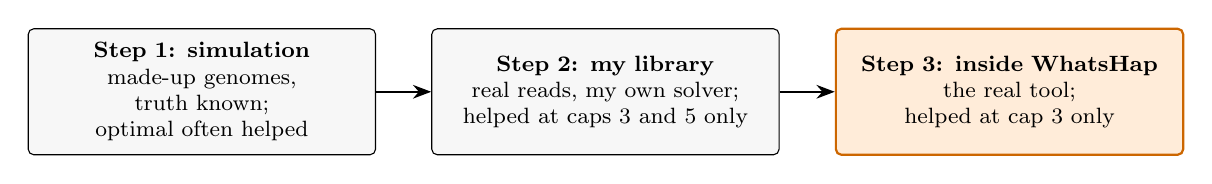
\begin{tikzpicture}[node distance=4mm and 7mm,
  st/.style={box,text width=4.2cm,minimum height=16mm}]
  \node[st] (s1) {\textbf{Step 1: simulation}\\made-up genomes, truth known;\\
    optimal often helped};
  \node[st,right=of s1] (s2) {\textbf{Step 2: my library}\\real reads, my own solver;\\
    helped at caps 3 and 5 only};
  \node[hl,text width=4.2cm,minimum height=16mm,right=of s2] (s3) {\textbf{Step 3: inside WhatsHap}\\the real tool;\\
    helped at cap 3 only};
  \draw[arr] (s1)--(s2); \draw[arr] (s2)--(s3);
\end{tikzpicture}
\caption{Three steps, from simulated data to the real tool.}
\label{fig:steps}
\end{figure}

\subsection{Step 1: simulation}

A simulator makes up two random copies, cuts reads from them, and adds
reading mistakes with base qualities. It can also add mistakes that the base
qualities do not warn about. Because we made the copies, the truth is known
exactly, and error rate, depth and site density can be changed one at a
time. Main findings (all on simulated data):

\begin{itemize}
\item The greedy rule kept 0.80 to 0.93 of the optimum over 12 settings
  (caps 3, 5, 8), and fell 8 to 13 per cent short on 2{,}000-site
  chromosomes. Closing the gap lowered switch error in 8 of 12 settings and
  raised it in 2.
\item Changing WhatsHap's score update back to the published rule turned 22
  to 27 blocks into 1 or 2 at cap 3.
\item A gap must count towards the cap, because the solver pays for it.
  Counting only the sites a read calls makes selection NP-hard, by a
  reduction from independent set.
\item A map over 210 settings shows when the MEC optimum is the truth: at
  depth 4 up to 3 to 10 per cent reading error, at depth 12 up to 10 to 20
  per cent.
\item Per-link margins (the cost of flipping a link) weaken as MEC and truth
  drift apart (correlation $-0.893$ over 130 settings). A posterior is a
  calibrated probability when base qualities are right (calibration error
  0.002 to 0.009), and 5 to 20 times worse when they are wrong.
\item Merging reads that share a copy before selection gave 1.9 to 4.8
  times fewer errors at caps 3 and 5, and merging plus a reselection loop
  about 11 times fewer. HapCHAT's merge threshold of $10^6$ was too strict
  ($10^3$ was 1.4 to 3.2 times better).
\item Orienting blocks with all reads by a second exact program
  (\enquote{two-level}) raised block N50 from 88 to 2{,}006\,kb. A flow that
  keeps blocks connected keeps 0.9997 of the optimum.
\item For a trio, one shared selection with a total cap of 9 matched
  WhatsHap's split of 15 per family.
\end{itemize}

\subsection{Step 2: real reads in my library}

My library phases the kept reads with its own exact dynamic program, so
any selector can be plugged in. Two phasings are compared only on links that
both phase. Links wrong in exactly one of the two are counted and checked
with the sign test (explained in Section~\ref{sec:result1}), and error bars
come from resampling 1\,Mb windows 2{,}000 times. The data: HG002 HiFi (28 to
39$\times$) and Nanopore (about 64$\times$), each also thinned to lower
depths; HG005 HiFi; 2{,}015{,}699 heterozygous sites on 21 chromosomes
(chromosome 20 was the pilot).

\paragraph{Pilot (chromosome 20).} The greedy reached 0.937 of the best
weight. HiFi reads made so few errors that the tests could not
tell the selectors apart (7 against 2 wrong links at cap 3). The reselection
loop, the best idea in simulation, made 17 wrong links against 2; every
extra one sat where two of its windows were stitched together, and a repair
brought it back to 2. The answer key itself had two wrong sites, confirmed
from the father's reads.

\paragraph{Genome-wide.} The table gives greedy's wrong links minus
optimal's wrong links, per 10{,}000 links, at full depth. A positive number
means optimal made fewer errors:

\begin{center}
\small
\begin{tabular}{@{}lrrr@{}}
\toprule
cap & HG002 HiFi & HG002 Nanopore & HG005 HiFi\\
\midrule
3 & $+0.50$ & $+8.81$ & $+0.41$\\
5 & $+0.04$ (not significant) & $+0.83$ & not significant\\
15 & $-0.01$ (not significant) & $+0.03$ (not significant) & not significant\\
\bottomrule
\end{tabular}
\end{center}

Lower depths showed the same pattern, stronger on Nanopore (up to
$+15.01$ at cap 3 and 10$\times$). So the choice of reads changes accuracy
at cap 3, on Nanopore also at cap 5, and never at cap 10 or 15. At cap 3 on
HiFi, the greedy left 7.6 per cent of links resting on a single kept read,
against 3.1 per cent for optimal, and such one-read links were wrong 11.25
against 1.49 times per 10{,}000. The best ideas from simulation did not help
on real reads. The loop was worse than plain optimal (354 against 56 wrong
links at cap 3), and merging helped on HiFi only at 10$\times$ (on Nanopore
at caps 3 and 5 at every depth). The simulation had used much higher error
rates than real HiFi reads have. The posterior margin did rank wrong links
well (area under the curve 0.961, where 1 is perfect and 0.5 is guessing).

\subsection{Step 3: the change inside WhatsHap}

A result in my own library might not hold in the real tool. So I swapped
one step inside \code{whatshap phase} and kept everything else as shipped
(Figure~\ref{fig:patch}).

\begin{figure}[h]
\centering
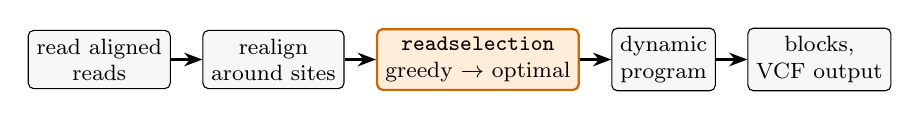
\begin{tikzpicture}[node distance=3mm and 4mm]
  \node[box] (a) {read aligned\\reads};
  \node[box,right=of a] (b) {realign\\around sites};
  \node[hl,right=of b] (c) {\code{readselection}\\greedy $\to$ optimal};
  \node[box,right=of c] (d) {dynamic\\program};
  \node[box,right=of d] (e) {blocks,\\VCF output};
  \foreach \x/\y in {a/b,b/c,c/d,d/e} \draw[arr] (\x)--(\y);
\end{tikzpicture}
\caption{\code{whatshap phase} 2.8. Only the orange step changes.}
\label{fig:patch}
\end{figure}

WhatsHap's \code{phase.py} calls a function named \code{readselection}. In
Python a module's functions can be replaced from outside, so swapping in my
function before WhatsHap starts makes \code{phase.py} call mine instead. This
is \code{benchmarks/whatshap\_exact.py}, slightly shortened:

\begin{lstlisting}
import whatshap.cli.phase as phase_module
from whatshap.__main__ import main as whatshap_main
from phasebudget.selection import select_optimal

def exact_readselection(readset, max_coverage, preferred_source_ids=None):
    positions = sorted({v.position for read in readset for v in read})
    index = {p: j for j, p in enumerate(positions)}
    reads = []
    for k, read in enumerate(readset):
        sites = sorted(index[v.position] for v in read)
        if len(sites) < 2:              # one site says nothing about phase
            continue
        weight = sum(v.quality for v in read)          # WhatsHap's own qualities
        reads.append((k, sites[0], sites[-1] + 1, weight))
    return select_optimal(reads, len(positions), max_coverage)

phase_module.readselection = exact_readselection   # the only change
whatshap_main()                                     # then run `whatshap phase`
\end{lstlisting}

The cap is set with WhatsHap's usual \code{-{}-internal-downsampling} option.

\subsection{Results inside WhatsHap}\label{sec:result1}

I ran stock and changed \code{whatshap phase} on HG002 (21 chromosomes, full
depth) at caps 3, 5 and 15, once with Nanopore reads (Test 1) and once with
HiFi reads. The short answer: the best choice of reads helps only when very
few reads are kept (Figure~\ref{fig:capbars}).

\begin{figure}[h]
\centering
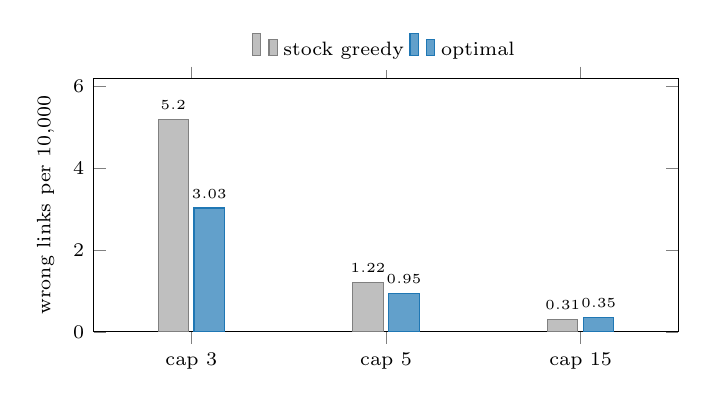
\begin{tikzpicture}
\begin{axis}[ybar,width=9cm,height=4.8cm,bar width=11pt,
  symbolic x coords={cap 3,cap 5,cap 15},xtick=data,ymin=0,ymax=6.2,
  ylabel={wrong links per 10{,}000},enlarge x limits=0.25,
  legend style={font=\scriptsize,draw=none,at={(0.5,1.03)},anchor=south,legend columns=2},
  nodes near coords,nodes near coords style={font=\tiny,/pgf/number format/fixed},
  tick label style={font=\scriptsize},label style={font=\scriptsize}]
\addplot[fill=gray!50,draw=gray] coordinates {(cap 3,5.204) (cap 5,1.215) (cap 15,0.310)};
\addplot[fill=keep!70,draw=keep] coordinates {(cap 3,3.029) (cap 5,0.947) (cap 15,0.346)};
\legend{stock greedy, optimal}
\end{axis}
\end{tikzpicture}
\caption{\code{whatshap phase} on HG002 Nanopore (Test 1). The best choice
of reads helps a lot at cap 3, and the gap disappears by cap 15.}
\label{fig:capbars}
\end{figure}

\paragraph{How the two runs are compared.} Most links are right in both
runs, so they say nothing about which selector is better. Only
\emph{discordant} links count: wrong in one run and right in the other. If
the selectors were equally good, each discordant link would fall on either
side like a fair coin. The \emph{sign test} checks this, at level $0.05/3$
because three caps are tested.

\begin{center}
\small
\begin{tabular}{@{}lcccc@{}}
\toprule
 & \multicolumn{2}{c}{wrong links per 10{,}000} & \multicolumn{2}{c}{discordant links}\\
 & stock & optimal & wrong only in stock / only in optimal & $p$\\
\midrule
\multicolumn{5}{@{}l}{\emph{Nanopore}}\\
cap 3 & 5.20 & \textbf{3.03} & 888 / 485 & $8.4\times10^{-28}$\\
cap 5 & 1.22 & 0.95 & 177 / 136 & 0.024\\
cap 15 & 0.31 & 0.35 & 16 / 25 & 0.21\\
\multicolumn{5}{@{}l}{\emph{HiFi}}\\
cap 3 & 0.55 & 0.41 & 66 / 46 & 0.072\\
cap 5 & & & 25 / 25 & \\
cap 15 & 0.17 & 0.20 & 9 / 9 & \\
\bottomrule
\end{tabular}
\end{center}

Only one result is significant: Nanopore at cap 3, where the best choice
removed 42 per cent of the errors. It also has a cost. Phased output comes
in blocks with no links between them, and block N50 (half of the phased
sequence lies in blocks at least this long) fell from 658 to 442\,kb at cap
3. The flow picks heavy reads and gives no credit to reads that join distant
sites.

\paragraph{Why only at cap 3.} Think of the reads over a link as a jury
voting cis or trans, each juror wrong with probability $q$. A jury of $i$
gets the majority wrong with probability
$f(i)=\Pr[\Bin(i,q)>i/2]+\tfrac12\Pr[\Bin(i,q)=i/2]$ (a coin breaks
ties~\cite{berend2005}), and $f$ drops fast as the jury grows
(Figure~\ref{fig:jury}). With 15 jurors, swapping one rarely changes the
verdict, so a slightly worse choice of reads costs almost nothing. With 3
jurors, one swap often decides it.

\begin{figure}[h]
\centering
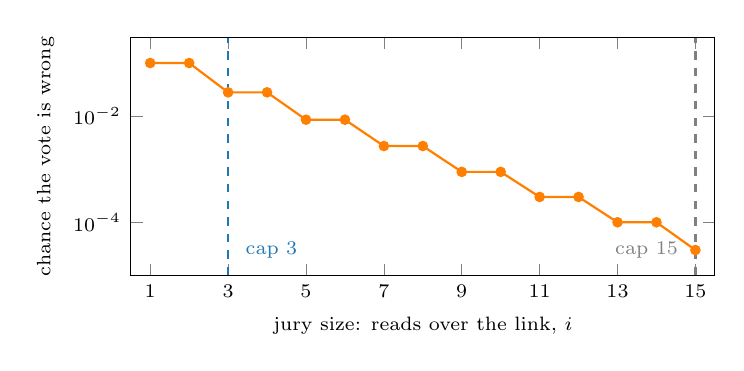
\begin{tikzpicture}
\begin{axis}[width=9cm,height=4.6cm,ymode=log,xmin=0.5,xmax=15.5,ymin=1e-5,ymax=0.3,
  xlabel={jury size: reads over the link, $i$},ylabel={chance the vote is wrong},
  tick label style={font=\scriptsize},label style={font=\scriptsize},xtick={1,3,5,7,9,11,13,15}]
\addplot[thick,orange,mark=*,mark size=1.5pt] coordinates {(1,0.1) (2,0.1) (3,0.028)
  (4,0.028) (5,0.00856) (6,0.00856) (7,0.00273) (8,0.00273) (9,0.00089) (10,0.00089)
  (11,0.0003) (12,0.0003) (13,0.0001) (14,0.0001) (15,0.00003)};
\draw[keep,thick,dashed] (axis cs:3,1e-5) -- (axis cs:3,0.3);
\draw[gray,thick,dashed] (axis cs:15,1e-5) -- (axis cs:15,0.3);
\node[font=\scriptsize,keep,anchor=west] at (axis cs:3.2,3e-5) {cap 3};
\node[font=\scriptsize,gray,anchor=east] at (axis cs:14.8,3e-5) {cap 15};
\end{axis}
\end{tikzpicture}
\caption{The vote model with each read wrong 10 per cent of the time
(illustration). Ties count as half wrong, so odd and even juries pair up.}
\label{fig:jury}
\end{figure}

I turned this \emph{vote model} into a numeric prediction of the gap for
the Nanopore and HG005 runs, using a read error rate measured on chromosome
20, with three pass rules. Two held: the predictions fell within a factor of
2 of the data, and the model beat three simple baselines (mean error 0.61
against 2.22 to 3.59). The third failed: in 3 of the cells (1 of 16 Nanopore
cells, both HG005 cap-3 cells) the prediction fell just below the 0.5 per
10{,}000 line used to decide whether the choice of reads changes accuracy.

\paragraph{Tied sites.} In my own library the cap-3 Nanopore gap first
looked much larger, 8.81 per 10{,}000. Most of it came from \emph{tied
sites}, where the kept reads weigh the same for both answers: my solver
guessed there, while \code{whatshap phase} leaves them unphased. Greedy left
1{,}640 ties and optimal 33. Leaving ties unphased cut the gap to 1.33, close
to the tool's 2.06. So a fair comparison must count what each method leaves
unanswered.

\paragraph{The phaser counts more.} On HG002 HiFi, stock WhatsHap at cap 15
made 0.165 errors per 10{,}000 links, LongPhase 0.150 and HiPhase 0.052
(both keep all reads). Changing the phaser changed errors more than changing
the choice of reads.

\paragraph{Other ideas tried on real reads.} All in the library, HG002 HiFi
unless stated:

\begin{itemize}
\item The reselection loop was worse than plain optimal at cap 3 (349
  against 5 discordant links).
\item Selection that minimises expected errors failed its HiFi pilot (96
  against 39). On Nanopore it was better at full depth and worse at
  10$\times$.
\item Two-level orientation raised block N50 at cap 3 from 112 to 234\,kb,
  but the new joins were wrong 4.1 to 5.8 times per 10{,}000 at 10$\times$,
  against 0.52 to 0.76.
\item Connected selection reached an N50 of 233\,kb with the same trade-off.
\item Weights from base qualities raised wrong links at cap 3 from 82 to
  142.
\item A posterior correction was not calibrated on the Nanopore test (2.36
  times the predicted wrong calls).
\item In family (pedigree) mode no test was supported. Every run had 2 to 8
  wrong links in about 164{,}200, and a two-sided sign test needs at least 6
  discordant links to reach 0.05, so two of the tests could never pass.
\end{itemize}

\paragraph{Answer to Question 1.} At the default cap of 15, WhatsHap's
greedy rule is good enough, although it is 4 to 7 per cent short of the best
weight: with 15 jurors, a slightly worse jury still votes right. At cap 3,
the best choice is more accurate but gives shorter blocks. Changing the
objective or the read weights gave no consistent gain.

%=====================================================================
\section{When to trust a link: the method}\label{sec:promise}
%=====================================================================

\subsection{The idea}

Picture an exam where wrong answers are costly (Figure~\ref{fig:exam}).
Student A answers all 100 questions and gets 10 wrong. Student B answers 80,
writes \enquote{not sure} for the other 20, and gets only 1 wrong. Student C
answers nothing. When B answers, you can rely on the answer.

\begin{figure}[h]
\centering
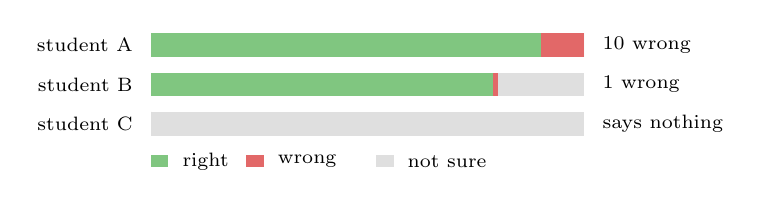
\begin{tikzpicture}[x=0.055cm,y=0.5cm,font=\scriptsize]
  \foreach \y/\n/\r/\w/\u in {2/A/90/10/0,1/B/79/1/20,0/C/0/0/100} {
    \node[anchor=east] at (-2,\y) {student \n};
    \fill[good!60] (0,\y-0.3) rectangle (\r,\y+0.3);
    \fill[bad!70] (\r,\y-0.3) rectangle (\r+\w,\y+0.3);
    \fill[gray!25] (\r+\w,\y-0.3) rectangle (100,\y+0.3);}
  \node[anchor=west] at (102,2) {10 wrong};
  \node[anchor=west] at (102,1) {1 wrong};
  \node[anchor=west] at (102,0) {says nothing};
  \fill[good!60] (0,-1.1) rectangle (4,-0.8); \node[anchor=west] at (5,-0.95) {right};
  \fill[bad!70] (22,-1.1) rectangle (26,-0.8); \node[anchor=west] at (27,-0.95) {wrong};
  \fill[gray!25] (52,-1.1) rectangle (56,-0.8); \node[anchor=west] at (57,-0.95) {\enquote{not sure}};
\end{tikzpicture}
\caption{Saying \enquote{not sure} on a few hard questions makes the rest
trustworthy.}
\label{fig:exam}
\end{figure}

The method does the same with any phaser's output: each link is marked
\emph{trust} or \emph{not sure}. Wrong trusted links must be rare, even on a
person the method has never seen; this is the \emph{promise}. Most links
should still be trusted. Figure~\ref{fig:trustflow} shows the procedure:
learn cutoffs on people whose true phase is known, then use them unchanged
on new people.

\begin{figure}[h]
\centering
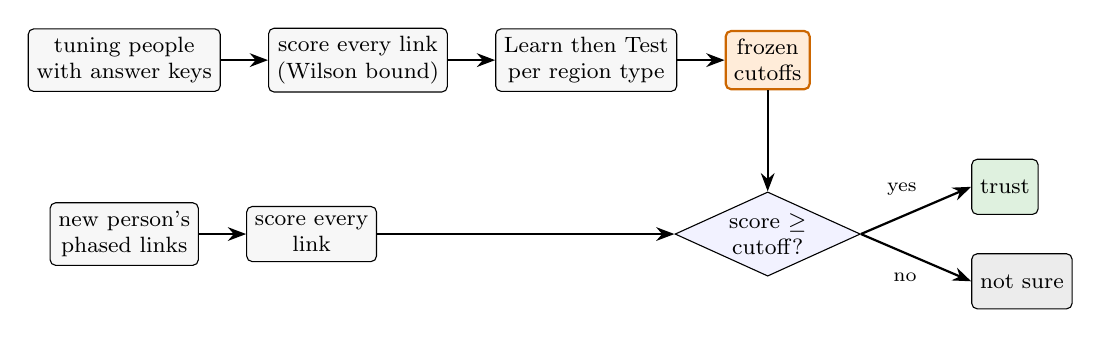
\begin{tikzpicture}[node distance=4mm and 6mm]
  \node[box] (cal) {tuning people\\with answer keys};
  \node[box,right=of cal] (sc) {score every link\\(Wilson bound)};
  \node[box,right=of sc] (ltt) {Learn then Test\\per region type};
  \node[hl,right=of ltt] (cut) {frozen\\cutoffs};
  \node[box,below=14mm of cal] (new) {new person's\\phased links};
  \node[box,right=of new] (sc2) {score every\\link};
  \node[dec] (q) at (cut |- sc2) {score $\ge$\\cutoff?};
  \node[box,fill=good!15,right=14mm of q,yshift=6mm] (t) {trust};
  \node[box,fill=gray!15,right=14mm of q,yshift=-6mm] (ns) {not sure};
  \draw[arr] (cal)--(sc); \draw[arr] (sc)--(ltt); \draw[arr] (ltt)--(cut);
  \draw[arr] (new)--(sc2); \draw[arr] (sc2)--(q);
  \draw[arr] (cut)--(q);
  \draw[arr] (q.east) -- node[above left,pos=0.6,font=\scriptsize]{yes} (t.west);
  \draw[arr] (q.east) -- node[below left,pos=0.6,font=\scriptsize]{no} (ns.west);
\end{tikzpicture}
\caption{Tune cutoffs on people with known answers, then apply them unchanged to new people.}
\label{fig:trustflow}
\end{figure}

\subsection{The score}

Each link needs a score that says how well the reads support it. Let $m$
be the number of reads covering both sites of the link, and $a$ the number
that agree with the phaser's answer. The plain share $a/m$ is a poor score:
it ranks 2 of 2 above 19 of 20, though 19 of 20 is stronger evidence. It
is like trusting a product with 5.0 stars from 2 reviews over one with 4.8
stars from 500. So I use a cautious version of the share, the lower end of
the Wilson interval~\cite{wilson1927}, with $z=2$ and $\hat q=a/m$:
\[
L(a,m)=\Big(\hat q+\tfrac{z^2}{2m}-z\sqrt{\tfrac{\hat q(1-\hat q)}{m}
+\tfrac{z^2}{4m^2}}\Big)\Big/\Big(1+\tfrac{z^2}{m}\Big).
\]
It is the smallest agreeing share that the data still make believable.
Few reads pull it down, and so do disagreeing reads
(Figure~\ref{fig:wilson}).

\begin{figure}[h]
\centering
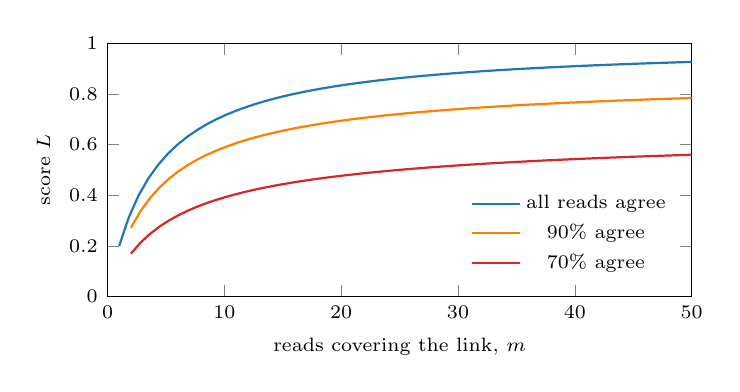
\begin{tikzpicture}
\begin{axis}[width=9cm,height=4.8cm,xmin=0,xmax=50,ymin=0,ymax=1,
  xlabel={reads covering the link, $m$},ylabel={score $L$},
  tick label style={font=\scriptsize},label style={font=\scriptsize},
  legend style={font=\scriptsize,draw=none,at={(0.98,0.05)},anchor=south east}]
\addplot[thick,keep,domain=1:50,samples=60] {x/(x+4)};
\addplot[thick,orange,domain=2:50,samples=60]
  {(0.9+2/x-2*sqrt(0.09/x+1/(x*x)))/(1+4/x)};
\addplot[thick,bad,domain=2:50,samples=60]
  {(0.7+2/x-2*sqrt(0.21/x+1/(x*x)))/(1+4/x)};
\legend{all reads agree, 90\% agree, 70\% agree}
\end{axis}
\end{tikzpicture}
\caption{The score grows with the number of reads, and drops when some reads
disagree.}
\label{fig:wilson}
\end{figure}

\begin{center}
\small
\begin{tabular}{@{}lccccccccc@{}}
\toprule
agreeing reads & 1/1 & 2/2 & 5/5 & 10/10 & 20/20 & 50/50 & 19/20 & 8/10 & 5/10\\
\midrule
score $L$ & 0.20 & 0.33 & 0.56 & 0.71 & 0.83 & 0.93 & 0.76 & 0.48 & 0.23\\
\bottomrule
\end{tabular}
\end{center}

\begin{lstlisting}
def wilson_lower(agree, reads, z=2.0):
    if reads == 0:
        return -1.0                                   # no read spans the link
    q = agree / reads
    centre = q + z * z / (2 * reads)
    spread = z * sqrt(q * (1 - q) / reads + z * z / (4 * reads * reads))
    return (centre - spread) / (1 + z * z / reads)    # ties broken by `reads`
\end{lstlisting}

The score uses only the reads, never the answer key, so it works on any
new sample. Reads are taken from the BAM file the way \code{whatshap phase}
takes them (realigned around each site, mapping quality at least 20), and
all reads are used, including those WhatsHap dropped. On HG002 HiFi the
score separated wrong links from right ones with an area under the curve of
0.998 (0.995 for the plain margin $a-(m-a)$). So ranking links is easy. The
hard part is choosing a cutoff $t$ with a stated error rate. A link is
trusted when its score is at least $t$.

\subsection{The promise counts 100\,kb stretches}

Errors come in clumps: one misplaced site breaks both of its links, and a
hard region gives several wrong links close together. Counting wrong links
one by one would treat a clump as many separate failures. So each chromosome
is cut into 100\,kb \emph{stretches}. A stretch is \emph{active} if it holds
at least one trusted link, and \emph{bad} if it holds at least one wrong
trusted link (Figure~\ref{fig:stretch}).

\begin{figure}[h]
\centering
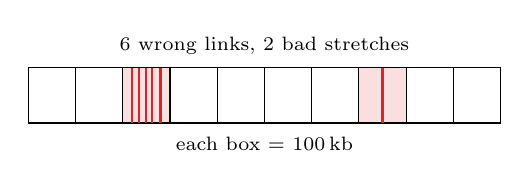
\begin{tikzpicture}[x=0.6cm,font=\scriptsize]
  \fill[bad!15] (2,0) rectangle (3,0.7);
  \fill[bad!15] (7,0) rectangle (8,0.7);
  \foreach \i in {0,...,9} \draw (\i,0) rectangle (\i+1,0.7);
  \foreach \x in {2.2,2.35,2.5,2.62,2.8} \draw[bad,thick] (\x,0) -- (\x,0.7);
  \draw[bad,thick] (7.5,0) -- (7.5,0.7);
  \node[above] at (5,0.75) {6 wrong links, 2 bad stretches};
  \node[below] at (5,-0.05) {each box = 100\,kb};
\end{tikzpicture}
\caption{Counting bad stretches instead of wrong links.}
\label{fig:stretch}
\end{figure}

\begin{definition}[The promise]
With probability at least $1-\delta$ over the tuning data, at most a share
$\beta$ of active stretches are bad. Defaults: $\beta=10^{-3}$, $\delta=0.05$;
tests also use $\beta=3\times10^{-4}$ and $3\times10^{-3}$.
\end{definition}

In words: among stretches with a trusted link, at most 1 in 1{,}000 has a
wrong one, and the chance that this promise is false is at most 5 per cent.
The promise also covers any cis/trans question between two sites in the same
stretch, since such an answer is wrong only if a link between them is wrong.
I chose 100\,kb because on Nanopore data, bad 10\,kb windows sat next to
each other more often than chance ($p=0.0005$), while bad 100\,kb stretches
did not (1 adjacent pair against 1.14 expected, $p=0.69$).

\subsection{Choosing the cutoff with Learn then Test}

The idea is to start with a very strict cutoff and loosen it one step at a
time, stopping the first time the evidence of safety is not strong enough.
The candidate cutoffs $t_1,t_2,\dots$ are the scores at which 50, 50.25,
\dots, 100 per cent of tuning links would be trusted, from strict to loose.
For each, count $N$ active and $K$ bad stretches and compute
$\pi=\Pr[\Bin(N,\beta)\le K]$: the chance of seeing this few bad stretches if
the true rate were as high as $\beta$. A small $\pi$ means the true rate is
probably below $\beta$. Walk from strict to loose, keep going while
$\pi\le\delta$, and stop at the first failure (Figure~\ref{fig:ltt} and the
table below).

\begin{figure}[h]
\centering
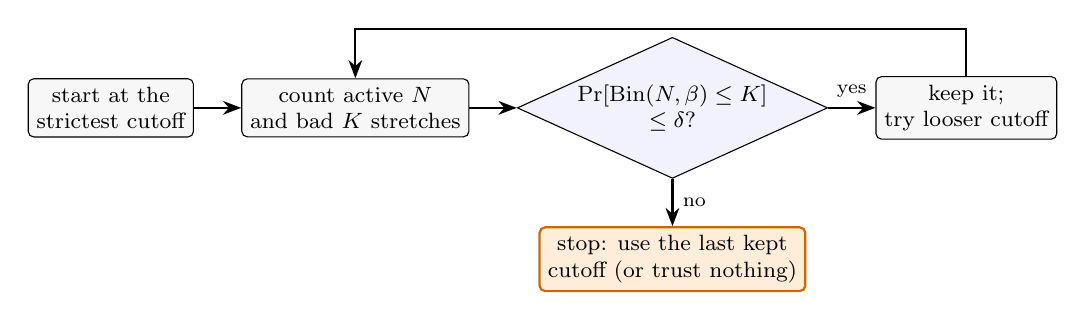
\begin{tikzpicture}[node distance=4mm and 6mm]
  \node[box] (s) {start at the\\strictest cutoff};
  \node[box,right=of s] (c) {count active $N$\\and bad $K$ stretches};
  \node[dec,right=of c] (d) {$\Pr[\Bin(N,\beta)\le K]$\\$\le\delta$?};
  \node[box,right=of d] (k) {keep it;\\try looser cutoff};
  \node[hl,below=6mm of d] (stop) {stop: use the last kept\\cutoff (or trust nothing)};
  \draw[arr] (s)--(c); \draw[arr] (c)--(d);
  \draw[arr] (d)--node[above,font=\scriptsize]{yes}(k);
  \draw[arr] (k.north) -- ++(0,6mm) -| (c.north);
  \draw[arr] (d)--node[right,font=\scriptsize]{no}(stop);
\end{tikzpicture}
\caption{Learn then Test, fixed-sequence form.}
\label{fig:ltt}
\end{figure}

\begin{center}
\small
\begin{tabular}{@{}rrrl@{}}
\toprule
cutoff & links trusted & bad stretches & clearly below $10^{-3}$?\\
\midrule
0.95 & 40\% & 0 of 4{,}000 & yes ($p=0.018$)\\
0.90 & 70\% & 1 of 7{,}000 & yes ($p=0.007$)\\
0.80 & 90\% & 3 of 9{,}000 & yes ($p=0.021$): \textbf{use this}\\
0.70 & 97\% & 40 of 9{,}700 & no: stop\\
\bottomrule
\end{tabular}

{\footnotesize Made-up numbers, for illustration.}
\end{center}

This is Learn then Test~\cite{ltt2025}. Because the order is fixed and the
walk stops at the first failure, the chance of ending on an unsafe cutoff is
at most $\delta$, even though many cutoffs are tried. It relies on three
assumptions: (1) tuning and test stretches come from the same population,
independently; (2) the order of cutoffs is fixed before any errors are seen;
(3) the answer key is right. Most later sections are about what happens
when assumption (1) fails.

\begin{proof}[Why the walk is safe]
Fix a candidate $t_g$ whose true rate $R(t_g)$ is above $\beta$. Given $N$,
the bad count $K$ is binomial with rate $R(t_g)>\beta$, so the chance that
$\Pr[\Bin(N,\beta)\le K]\le\delta$ is at most $\delta$: each p-value is
valid. The order is fixed, so the first unsafe candidate $g^*$ is fixed
too. Ending on an unsafe cutoff means the walk passed $g^*$, which means its
p-value was at most $\delta$. That has probability at most $\delta$.
\end{proof}

\paragraph{Restricting the links.} Suppose a fixed rule, which never looks
at the answer key, marks some links \enquote{eligible}. Running the same procedure
on eligible links only gives a promise for eligible links, and says nothing
about the others. Section~\ref{sec:keys} uses this fact to explain why
pooling 21 people failed.

\subsection{One cutoff per region type}\label{sec:regions}

Some parts of the genome are much harder to phase than others. A single
cutoff for the whole genome must be strict enough for the hardest part, so
it is too strict for the easy parts. As a school sets one pass
mark per subject, the method sets one cutoff per \emph{region type}, using
GIAB's maps of difficult regions~\cite{dwarshuis2024}
(Figure~\ref{fig:regions}). Each link gets the first type in this list that
applies:

\begin{center}
\small
\begin{tabular}{@{}lp{11.5cm}@{}}
\toprule
type & meaning\\
\midrule
\grp{indel} & a site is an insertion or deletion, not a one-letter change\\
\grp{segdup} & segmental duplication: a long stretch copied elsewhere in the genome\\
\grp{lowmap} & low mappability: looks like some other place\\
\grp{tandem} & tandem repeat, such as \dna{CACACACA\dots}\\
\grp{easy} & both sites outside every difficult region\\
\grp{difficult} & mildly hard, none of the above\\
\bottomrule
\end{tabular}
\end{center}

\begin{figure}[h]
\centering
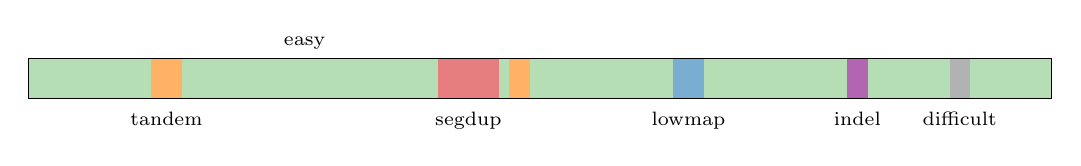
\begin{tikzpicture}[x=0.13cm,font=\scriptsize]
  \fill[good!35] (0,0) rectangle (100,0.5);
  \foreach \a/\b/\c in {12/15/orange,40/46/bad,47/49/orange,63/66/keep,80/82/violet,90/92/gray}
    \fill[\c!60] (\a,0) rectangle (\b,0.5);
  \draw (0,0) rectangle (100,0.5);
  \node[anchor=north] at (13.5,-0.05) {tandem};
  \node[anchor=north] at (43,-0.05) {segdup};
  \node[anchor=north] at (64.5,-0.05) {lowmap};
  \node[anchor=north] at (81,-0.05) {indel};
  \node[anchor=north] at (91,-0.05) {difficult};
  \node[anchor=south] at (27,0.5) {easy};
\end{tikzpicture}
\caption{A made-up stretch of chromosome: mostly easy, with scattered hard
regions. Each region type gets its own cutoff.}
\label{fig:regions}
\end{figure}

The hard types are mostly repeats. A read from a similar copy elsewhere in
the genome gets placed at the wrong spot, and it lands there in every
sample, so adding more reads does not outvote it. A type where no cutoff
passes trusts nothing: every link there is \enquote{not sure}.

Figure~\ref{fig:worked} follows two links through the whole method.

\begin{figure}[h]
\centering
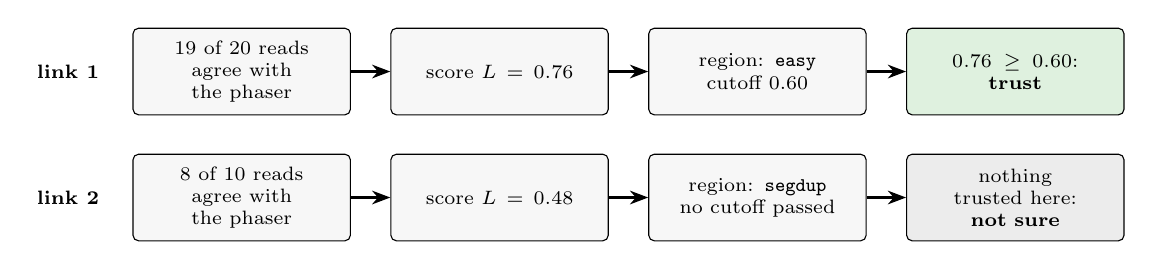
\begin{tikzpicture}[node distance=2.5mm and 5mm,
  c/.style={box,text width=2.55cm,font=\scriptsize,minimum height=11mm}]
  \node[font=\scriptsize\bfseries,anchor=east] at (-0.3,0) {link 1};
  \node[c,anchor=west] (a1) at (0,0) {19 of 20 reads\\agree with the phaser};
  \node[c,right=of a1] (b1) {score $L=0.76$};
  \node[c,right=of b1] (c1) {region: \grp{easy}\\cutoff 0.60};
  \node[c,right=of c1,fill=good!15] (d1) {$0.76\ge0.60$:\\\textbf{trust}};
  \node[font=\scriptsize\bfseries,anchor=east] at (-0.3,-1.6) {link 2};
  \node[c,anchor=west] (a2) at (0,-1.6) {8 of 10 reads\\agree with the phaser};
  \node[c,right=of a2] (b2) {score $L=0.48$};
  \node[c,right=of b2] (c2) {region: \grp{segdup}\\no cutoff passed};
  \node[c,right=of c2,fill=gray!15] (d2) {nothing trusted here:\\\textbf{not sure}};
  \foreach \x/\y in {a1/b1,b1/c1,c1/d1,a2/b2,b2/c2,c2/d2} \draw[arr] (\x)--(\y);
\end{tikzpicture}
\caption{Two links through the method. The scores are real values of the
formula above; the cutoff 0.60 is an illustration.}
\label{fig:worked}
\end{figure}

\subsection{Testing on a new person}

The cutoffs are frozen and applied to test people. Results are split into
\emph{cells}: one test person, coverage, phaser, error target $\beta$ and
region type. In a cell with $n$ active and $k$ bad stretches, compute
$p=\Pr[\Bin(n,\beta)\ge k]$, the chance of this many bad stretches if the
promise were exactly met. The cell \emph{breaks} if
$p<0.05/(\text{number of cells})$ (the Bonferroni correction).

The level is strict because with many cells, some look bad by luck: if 72 people
each toss a fair coin 5 times, someone gets five heads with probability
$1-(31/32)^{72}\approx 0.90$. Example with 72 cells (level 0.0007),
$n=3{,}119$ and $\beta=10^{-3}$, so about 3 bad stretches are expected:
$k=2$ gives $p=0.82$, the promise holds; $k=12$ gives $p\approx0.0001$, it
breaks. A type that trusts nothing can never break, so every result also
reports how much was trusted.

%=====================================================================
\section{Results on new people}\label{sec:held}
%=====================================================================

Each test tunes the cutoffs on some people and checks them, unchanged, on
others. Figure~\ref{fig:bars} counts the cells that broke. In short: one
cutoff for the whole genome failed; one cutoff per region type held in every
easy cell, and in hard regions it held mostly by trusting nothing; pooling 21
people got hard regions trusted, but there the promise broke.

\begin{figure}[h]
\centering
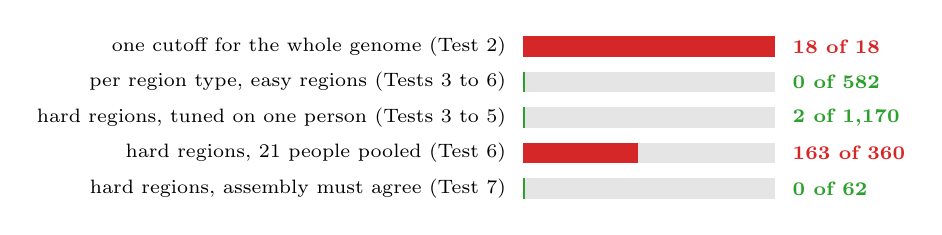
\begin{tikzpicture}[x=3.2cm]
  \failbar{0}{one cutoff for the whole genome (Test 2)}{1}{18 of 18}{bad}
  \failbar{-0.45}{per region type, easy regions (Tests 3 to 6)}{0}{0 of 582}{good}
  \failbar{-0.90}{hard regions, tuned on one person (Tests 3 to 5)}{0.0017}{2 of 1{,}170}{good}
  \failbar{-1.35}{hard regions, 21 people pooled (Test 6)}{0.453}{163 of 360}{bad}
  \failbar{-1.80}{hard regions, assembly must agree (Test 7)}{0}{0 of 62}{good}
\end{tikzpicture}
\caption{Test cells that broke, on people never used for tuning.}
\label{fig:bars}
\end{figure}

\paragraph{One cutoff for the whole genome (Test 2).} Cutoffs tuned on HG002
Nanopore broke in all 18 cells on HG001, at 3.6 to 42 times $\beta$. Part of
this was the 2017 answer key, which is wrong at about 1{,}700 sites: on
GIAB's own HG001 sites (88 per cent of links), WhatsHap lost 98.5 per cent
of its errors and no cell broke. The rest of the errors sat in hard regions,
and one cutoff strict enough for them trusts nothing anywhere else. One
cutoff per region type fixes this: it trusted 65.5 to 66.6 per cent of
WhatsHap's links on the relatives (Test 3) and 60 per cent on HG001 (Test
4), where one cutoff trusted none.

\paragraph{The answer key for the HPRC people.} Errors in the key add to
every cell, so the key must be much more accurate than the promise. An HPRC
person's assembly alone disagreed with parent-based keys in 278 of 47{,}737
easy stretches, which is too many. So the key labels a link only where the
assembly and the parents agree. Checked on NA12878, this key was accurate
enough (error at most $\beta/3$) only in easy and difficult regions, so Test
5 scores only those cells.

\paragraph{Easy regions (Tests 3 to 6).} All 582 easy cells held, across the
relatives, HG005, a newer basecaller and the 39 HPRC people. The cutoffs
still trusted 99.56 to 100 per cent of easy links on the relatives and 99.75
to 99.96 per cent per HPRC person. They were tuned on one European person
and held just as well for African, admixed American and East Asian people.

\paragraph{Hard regions, tuned on one person (Tests 3 to 5).} 1{,}168 of
1{,}170 cells held, mostly because nothing was trusted: \grp{segdup} trusted
no link in all 108 relative cells, and WhatsHap \grp{indel} none in Tests 3
and 4. This left 30 per cent of WhatsHap's links untrusted on the relatives,
against 5 per cent of LongPhase's, because WhatsHap phases many indel links
that the reads do not settle (on HG001, 2{,}834 indel links were wrong only
for WhatsHap and 106 only for LongPhase). The two breaks were WhatsHap
\grp{lowmap} cells on HG001. There most reads backed the wrong answer
(typically 15 of 21), the mark of reads from a similar copy elsewhere.

\paragraph{Pooling 21 people (Test 6).} Tuning on HG002 and 20 HPRC people
raised the trusted share of \grp{segdup} links on the five family members
from 0 to 82 per cent (\grp{tandem} from 42 to 86, \grp{indel} from 0 to
45). But 163 of 360 hard cells broke, \grp{segdup} worst (71 of 75 trusting
cells), with bad-stretch rates up to $3\times10^{-2}$. Easy and difficult
cells still held. Section~\ref{sec:keys} explains the breaks;
Section~\ref{sec:floor} first shows why one person is never enough.

%=====================================================================
\section{Why one person is not enough: a lower bound}\label{sec:floor}
%=====================================================================

\paragraph{Coin picture.} Suppose you want to show that a coin lands heads
less than once in 1{,}000 tosses. You must toss it about 3{,}000 times and
see no head at all. This is the \enquote{rule of three}: after $n$ clean trials,
the 95 per cent upper bound on the rate is about $3/n$. With fewer tosses
the claim cannot be shown, even if no head appears.

\paragraph{For Learn then Test.} The walk can only pass if its strictest
cutoff passes, and even with zero bad stretches,
$\Pr[\Bin(N,\beta)\le K]\ge(1-\beta)^N$. So a region type needs at least
\[
N^*(\beta,\delta)=\Big\lceil\frac{\ln\delta}{\ln(1-\beta)}\Big\rceil\approx
\frac{\ln(1/\delta)}{\beta}
\]
active stretches: 998, 2{,}995 and 9{,}985 at $\beta=3\times10^{-3}$, $10^{-3}$,
$3\times10^{-4}$ ($\delta=0.05$).

\begin{theorem}[Label floor]
A method sees $n$ labelled stretches of one sequencing batch, each bad
independently with probability $R$, plus any data whose distribution does not
depend on $R$. If it promises $\beta$ falsely with probability $\le\delta$
whenever $R>\beta$, and promises with probability $\ge p>\delta$ when $R=0$,
then $(1-\beta)^n p\le\delta$.
\end{theorem}

\begin{proof}[Idea]
Let $Z$ = all $n$ stretches clean. If $R=0$, $Z$ always happens, so the method
promises with probability $\ge p$ given $Z$. Given $Z$, the data look the same
whether $R=0$ or $R$ is just above $\beta$. For such $R$, $Z$ has probability
about $(1-\beta)^n$, so a false promise has probability $\ge(1-\beta)^n p$,
which must be $\le\delta$.
\end{proof}

\begin{figure}[h]
\centering
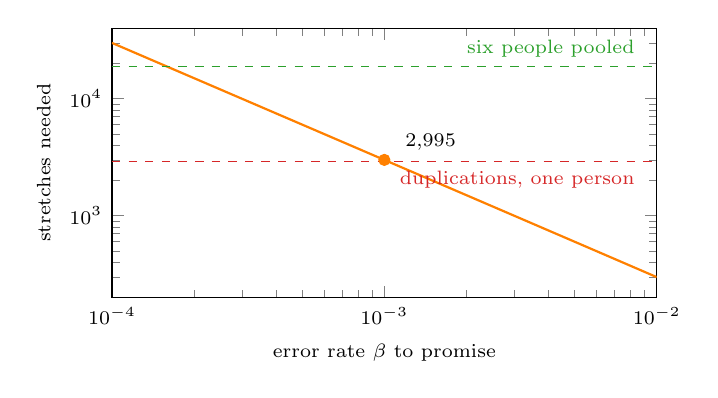
\begin{tikzpicture}
\begin{axis}[width=8.5cm,height=5cm,xmode=log,ymode=log,
  xmin=1e-4,xmax=1e-2,ymin=200,ymax=40000,
  xlabel={error rate $\beta$ to promise},ylabel={stretches needed},
  tick label style={font=\scriptsize},label style={font=\scriptsize}]
\addplot[domain=1e-4:1e-2,samples=60,thick,orange] {ln(20)/(x+x^2/2+x^3/3)};
\addplot[only marks,mark=*,orange] coordinates {(1e-3,2995)};
\node[font=\scriptsize,anchor=south west] at (axis cs:1.1e-3,2995) {2{,}995};
\addplot[dashed,bad,domain=1e-4:1e-2] {2900};
\node[font=\scriptsize,bad,anchor=north east] at (axis cs:9e-3,2900) {duplications, one person};
\addplot[dashed,good,domain=1e-4:1e-2] {18667};
\node[font=\scriptsize,good,anchor=south east] at (axis cs:9e-3,18667) {six people pooled};
\end{axis}
\end{tikzpicture}
\caption{The floor $N^*$ at $\delta=0.05$, against the data available.}
\label{fig:floor}
\end{figure}

The theorem covers every method that keeps the promise, so a different
statistical method would need the same amount of data.

\paragraph{Consequence.} One person at 30$\times$ has about 2{,}900 active
\grp{segdup} stretches (2{,}868 and 2{,}924 on HG002 Nanopore), just below
2{,}995 (Figure~\ref{fig:floor}). So no method can promise $10^{-3}$ in
duplications from one person. Six people give 18{,}667, but Test 6 showed
that pooling alone broke. The bound also says that a new
sequencing batch needs labels at genome scale (Section~\ref{sec:parents}).

%=====================================================================
\section{A second opinion from an assembly}\label{sec:assembly}
%=====================================================================

A phaser first places every read on the reference genome, then phases what
it finds there. In a duplicated region this goes wrong: a read from one copy
of the repeat can be placed on the other copy (Figure~\ref{fig:repeat}). An
\emph{assembly} skips the reference. hifiasm~\cite{cheng2021} overlaps the
reads with each other, like a jigsaw, and rebuilds both copies directly;
dipcall~\cite{li2018} then lines the rebuilt copies up against the reference
and reads off the sites and their phase. It works differently from a
phaser, so it usually fails in different places, and it can be used as a
second opinion.

\begin{figure}[h]
\centering
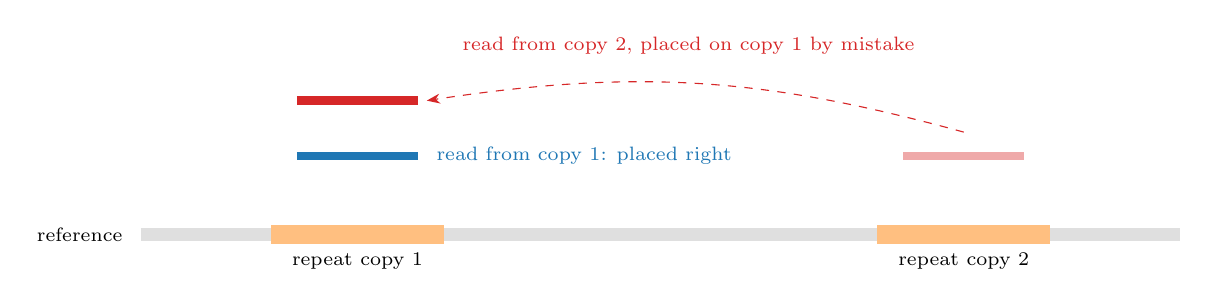
\begin{tikzpicture}[x=0.11cm,font=\scriptsize]
  \draw[line width=5pt,gray!25] (0,0) -- (120,0);
  \fill[orange!50] (15,-0.12) rectangle (35,0.12);
  \fill[orange!50] (85,-0.12) rectangle (105,0.12);
  \node[below=3pt] at (25,0) {repeat copy 1};
  \node[below=3pt] at (95,0) {repeat copy 2};
  \node[anchor=east] at (-1,0) {reference};
  \draw[line width=3pt,keep] (18,1.0) -- (32,1.0);
  \node[keep,anchor=west] at (33,1.0) {read from copy 1: placed right};
  \draw[line width=3pt,bad] (18,1.7) -- (32,1.7);
  \draw[bad,-{Stealth},dashed] (95,1.3) to[bend right=12] (33,1.7);
  \draw[line width=3pt,bad!40] (88,1.0) -- (102,1.0);
  \node[bad,anchor=west] at (36,2.4) {read from copy 2, placed on copy 1 by mistake};
\end{tikzpicture}
\caption{Why repeats fool a phaser. A read from one copy of a repeat looks
almost the same as the other copy, so it can be placed in the wrong spot.
More reads do not help, because every sample makes the same mistake.}
\label{fig:repeat}
\end{figure}

\begin{figure}[h]
\centering
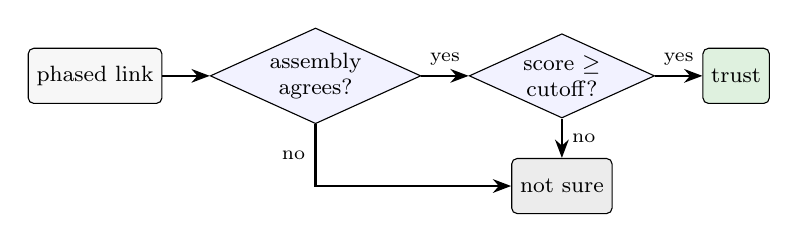
\begin{tikzpicture}[node distance=4mm and 6mm]
  \node[box] (l) {phased link};
  \node[dec,right=of l] (a) {assembly\\agrees?};
  \node[dec,right=of a] (s) {score $\ge$\\cutoff?};
  \node[box,fill=good!15,right=of s] (t) {trust};
  \node[box,fill=gray!15,below=5mm of s] (n) {not sure};
  \draw[arr] (l)--(a); \draw[arr] (a)--node[above,font=\scriptsize]{yes}(s);
  \draw[arr] (s)--node[above,font=\scriptsize]{yes}(t);
  \draw[arr] (a) |- node[pos=0.25,left,font=\scriptsize]{no} (n);
  \draw[arr] (s)--node[right,font=\scriptsize]{no}(n);
\end{tikzpicture}
\caption{The assembly rule. Cutoffs are tuned on agreeing links only.}
\label{fig:asm}
\end{figure}

The rule (Figure~\ref{fig:asm}): trust a link only if the assembly gives
the same answer \emph{and} the read score passes its cutoff. The assembly \emph{relates} two sites when both lie on the same
pair of rebuilt pieces, inside dipcall's confident region. A link
\emph{agrees} when the assembly relates it the same way as the phaser.

\begin{lstlisting}
def trusted(link, cutoff, assembly):
    relation = assembly.relation(link.site1, link.site2)   # "cis", "trans" or None
    if relation != link.phaser_relation:
        return False                                        # no second opinion
    return score(link) >= cutoff[link.region_type]
\end{lstlisting}

\begin{center}
\small
\begin{tabular}{@{}lrrr@{}}
\toprule
NA12877, \grp{segdup}, WhatsHap & links & wrong & about 1 in\\
\midrule
phaser and assembly agree & 87{,}000 & 6 & 15{,}000\\
all other links & 24{,}000 & 1{,}147 & 21\\
\bottomrule
\end{tabular}
\end{center}

When the two agree, a link is wrong about once in 15{,}000; otherwise
about once in 21. All 6 errors among agreeing links were wrong in the
assembly too, so the two methods are not fully independent, and the
statistical promise is still needed on top.

\paragraph{First evidence (HG002).} On HG002 HiFi, an assembly
from HG002's own reads (no parents) was right on all 478 hard-region links
that WhatsHap got wrong and the assembly phased. It agreed with the phaser on
91 to 99 per cent of links per region type. Among agreeing links, 0 of about
53{,}000 \grp{segdup} links were wrong; all 309 wrong WhatsHap \grp{segdup}
links lay among the few the assembly did not confirm. But on its own the
assembly is not a good key: it had 2{,}131 wrong of 1{,}249{,}172 easy
links, too many errors for an answer key.

\paragraph{Test 7.} Tuning pooled the agreeing links of six people (HG002
and the five family children), giving 18{,}667 (WhatsHap) and 18{,}736
(LongPhase) \grp{segdup} stretches, above the floor. Test people: NA12877,
the family's father; and HG005, unrelated, East Asian, sequenced by another
lab. NA12877 shares DNA with the children, so HG005 is the main test on
someone unrelated.

\begin{figure}[h]
\centering
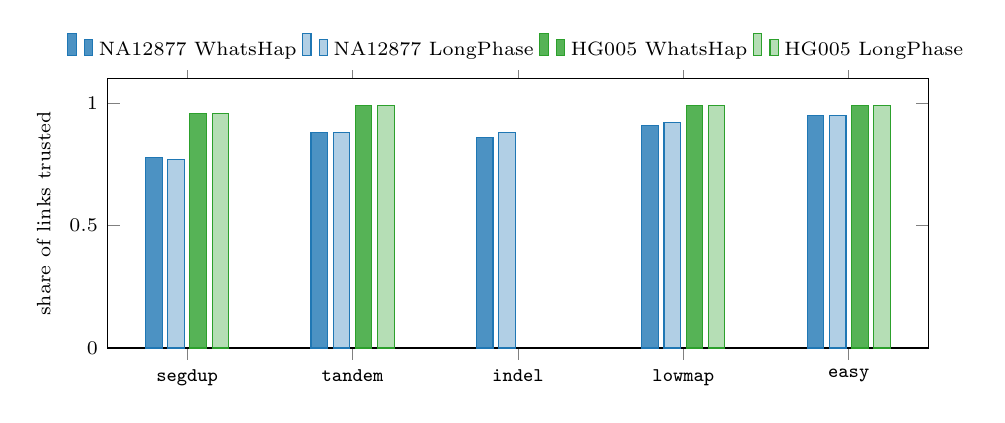
\begin{tikzpicture}
\begin{axis}[ybar,width=12cm,height=5cm,bar width=6pt,ymin=0,ymax=1.1,
  symbolic x coords={segdup,tandem,indel,lowmap,easy},xtick=data,
  xticklabel style={font=\scriptsize\ttfamily},
  ylabel={share of links trusted},enlarge x limits=0.12,
  legend style={font=\scriptsize,draw=none,at={(0.5,1.03)},anchor=south,legend columns=4},
  tick label style={font=\scriptsize},label style={font=\scriptsize}]
\addplot[fill=keep!80,draw=keep] coordinates {(segdup,0.78) (tandem,0.88) (indel,0.86) (lowmap,0.91) (easy,0.95)};
\addplot[fill=keep!35,draw=keep] coordinates {(segdup,0.77) (tandem,0.88) (indel,0.88) (lowmap,0.92) (easy,0.95)};
\addplot[fill=good!80,draw=good] coordinates {(segdup,0.96) (tandem,0.99) (lowmap,0.99) (easy,0.99)};
\addplot[fill=good!35,draw=good] coordinates {(segdup,0.96) (tandem,0.99) (lowmap,0.99) (easy,0.99)};
\legend{NA12877 WhatsHap, NA12877 LongPhase, HG005 WhatsHap, HG005 LongPhase}
\end{axis}
\end{tikzpicture}
\caption{Test 7: share of links trusted at $\beta=10^{-3}$ with the assembly
rule. Without the rule, the same pool trusted no \grp{segdup} link in any of
the four cells. HG005 has no \grp{indel} bars because its answer key has
single-letter sites only.}
\label{fig:k1b}
\end{figure}

\begin{figure}[h]
\centering
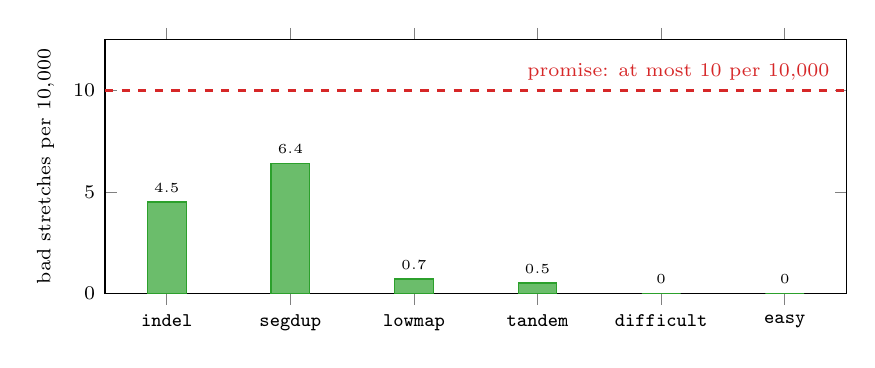
\begin{tikzpicture}
\begin{axis}[ybar,width=11cm,height=4.8cm,bar width=14pt,ymin=0,ymax=12.5,
  symbolic x coords={indel,segdup,lowmap,tandem,difficult,easy},xtick=data,
  xticklabel style={font=\scriptsize\ttfamily},
  ylabel={bad stretches per 10{,}000},enlarge x limits=0.1,
  nodes near coords,nodes near coords style={font=\tiny,/pgf/number format/fixed},
  tick label style={font=\scriptsize},label style={font=\scriptsize}]
\addplot[fill=good!70,draw=good] coordinates {(indel,4.5) (segdup,6.4) (lowmap,0.7) (tandem,0.5) (difficult,0) (easy,0)};
\draw[bad,thick,dashed] (rel axis cs:0,0.8) -- (rel axis cs:1,0.8);
\node[bad,font=\scriptsize,anchor=south east] at (rel axis cs:0.99,0.8) {promise: at most 10 per 10{,}000};
\end{axis}
\end{tikzpicture}
\caption{Test 7, NA12877, WhatsHap, $\beta=10^{-3}$: the share of stretches
with a wrong trusted link, per region type, on a person the cutoffs had
never seen. Every bar is under the promised rate. Counts: \grp{indel} 10 of
21{,}995 stretches, \grp{segdup} 2 of 3{,}119, \grp{lowmap} 1 of 13{,}833,
\grp{tandem} 1 of 20{,}118, \grp{difficult} 0 of 17{,}070, \grp{easy} 0 of
22{,}688.}
\label{fig:k1brate}
\end{figure}

All three predictions held: no cell broke (62 of 72 had a trusted
stretch; smallest $p=0.82$, NA12877 WhatsHap \grp{segdup}: 2 bad of 3{,}119),
and \grp{segdup} passed $10^{-3}$ for both phasers (not $3\times10^{-4}$).
Figure~\ref{fig:k1b} shows the trusted shares, and Figure~\ref{fig:k1brate}
shows that the error rate stayed under the target in every region type. The
same pool without the agreement rule broke no cell either, but it trusted
nothing in \grp{segdup} and nothing in WhatsHap's \grp{indel}. The assembly
rule is what lets these types be trusted at all.

%=====================================================================
\section{Why pooling 21 people failed}\label{sec:keys}
%=====================================================================

The 20 HPRC people in the Test 6 pool had no near-perfect key. A key from
their assembly alone was too noisy (278 of 47{,}737 easy stretches disagreed
with a parent-based key on HG002 and HG005). So the key labelled a link only
where the assembly and the parents (1000 Genomes genotypes) gave the same
answer (Figure~\ref{fig:key}). Two methods agree mostly where phasing is
easy.

\begin{figure}[h]
\centering
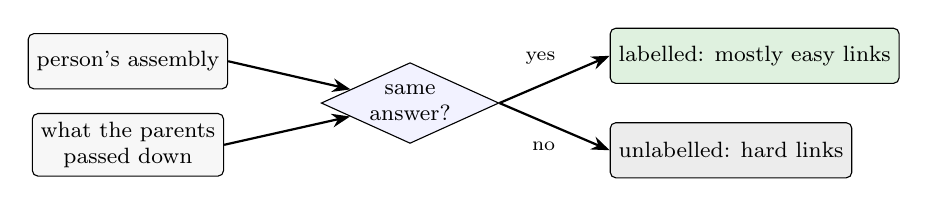
\begin{tikzpicture}[node distance=3mm and 6mm]
  \node[box] (as) {person's assembly};
  \node[box,below=of as] (pa) {what the parents\\passed down};
  \node[dec,right=12mm of $(as.east)!0.5!(pa.east)$] (ag) {same\\answer?};
  \node[box,fill=good!15,right=14mm of ag,yshift=6mm] (lab) {labelled: mostly easy links};
  \node[box,fill=gray!15,right=14mm of ag,yshift=-6mm] (un) {unlabelled: hard links};
  \draw[arr] (as.east)--(ag); \draw[arr] (pa.east)--(ag);
  \draw[arr] (ag.east)--node[above left,pos=0.6,font=\scriptsize]{yes}(lab.west);
  \draw[arr] (ag.east)--node[below left,pos=0.6,font=\scriptsize]{no}(un.west);
\end{tikzpicture}
\caption{How the pooled answer key was built, and what it kept.}
\label{fig:key}
\end{figure}

On HG002, where a near-perfect key exists, I built a key of this kind and
checked what it covers (Figure~\ref{fig:labshare}). It labels 0.75 of
\grp{easy} links, 0.66 of \grp{lowmap}, 0.46 to 0.49 of \grp{tandem} and
\grp{segdup}, and no \grp{indel} links. The links it skips are the hard
ones: over the three
repeat types at 30$\times$, all links were wrong 79 times as often as
labelled links for WhatsHap ($4.7\times10^{-3}$ against $5.9\times10^{-5}$),
and 12 times as often for LongPhase. So the cutoffs were tuned on
easy-looking links and then tested on all links. It is like setting a pass
mark using only the questions two teachers marked the same way, then
applying it to every question.

\begin{figure}[h]
\centering
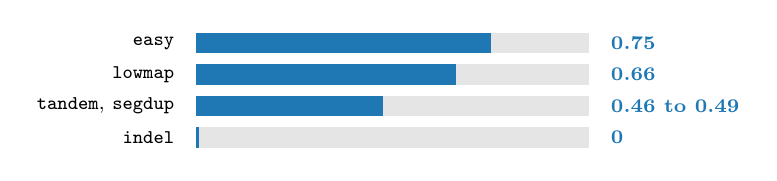
\begin{tikzpicture}[x=5cm]
  \failbar{0}{\grp{easy}}{0.75}{0.75}{keep}
  \failbar{-0.4}{\grp{lowmap}}{0.66}{0.66}{keep}
  \failbar{-0.8}{\grp{tandem}, \grp{segdup}}{0.475}{0.46 to 0.49}{keep}
  \failbar{-1.2}{\grp{indel}}{0}{0}{keep}
\end{tikzpicture}
\caption{Share of HG002's links that an \enquote{assembly and parents agree} key
labels. The harder the region, the less it covers.}
\label{fig:labshare}
\end{figure}

\paragraph{Three explanations, checked.} Three causes could explain the
breaks: (1) the key picks easy links; (2) the family was sequenced in a
different batch; (3) stretches of different people at the same place are not
independent. For each family child I built a key of the pool's kind and
rescored Test 6's frozen cutoffs (Figure~\ref{fig:keybars}).

\begin{figure}[h]
\centering
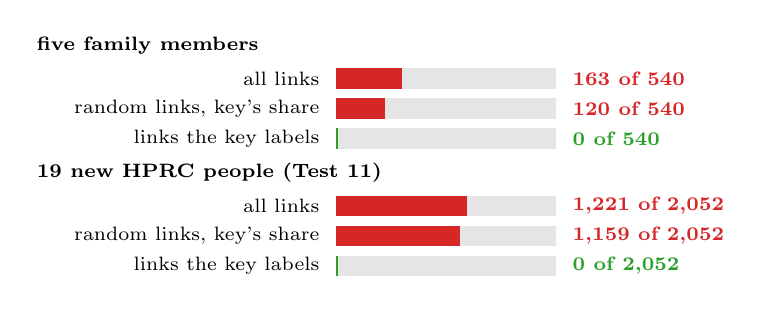
\begin{tikzpicture}[x=2.8cm]
  \node[anchor=west,font=\scriptsize\bfseries] at (-1.4,0.42) {five family members};
  \failbar{0}{all links}{0.302}{163 of 540}{bad}
  \failbar{-0.38}{random links, key's share}{0.222}{120 of 540}{bad}
  \failbar{-0.76}{links the key labels}{0}{0 of 540}{good}
  \node[anchor=west,font=\scriptsize\bfseries] at (-1.4,-1.2) {19 new HPRC people (Test 11)};
  \failbar{-1.62}{all links}{0.595}{1{,}221 of 2{,}052}{bad}
  \failbar{-2.0}{random links, key's share}{0.565}{1{,}159 of 2{,}052}{bad}
  \failbar{-2.38}{links the key labels}{0}{0 of 2{,}052}{good}
\end{tikzpicture}
\caption{The same pooled cutoffs, cells that broke.}
\label{fig:keybars}
\end{figure}

The \enquote{random links} row is the control. If the breaks vanished on key
links only because fewer links means less power to detect a break, random
links at the same share would also stop breaking. They kept breaking. So the
cause is which links are tested. Batch did not explain it: on key links
the children were not more error-prone than the pool (WhatsHap \grp{segdup}
$2.3\times10^{-4}$ against $7.6\times10^{-4}$). Shared error places did exist (0.85
of a child's bad \grp{segdup} stretches were bad in a sibling) but did not
decide the result.

In terms of Section~\ref{sec:promise}, the answer key worked as a rule
marking links eligible, so the cutoffs controlled errors among labelled
links only.

\paragraph{Replication on new people (Test 11).} The same effect was
checked on 19 HPRC people not in the pool, with three pass rules (scoring
key: each person's assembly; \enquote{key links}: those the consensus labels).

\begin{itemize}
\item In at least 17 of 19 people, the repeat-type error on all links should
  be more than 3 times that on key links. This held in 19 of 19, with ratios
  14 to 103.
\item At least 15 people should have a broken hard cell on all links. This
  held in 19 of 19, with 1{,}221 of 2{,}052 cells broken.
\item No cell should break on key links. None did (0 of 2{,}052), while
  random links of the same share broke 1{,}159.
\end{itemize}

One limit: off the consensus, the assembly is the only key, so its errors
count as phaser errors. Test 12 uses a family key with no assembly in it.
The same logic explains Test 7: tuning and testing both used agreeing links,
chosen by the same rule.

%=====================================================================
\section{Gene-level calls}\label{sec:genes}
%=====================================================================

A doctor's question is about two variants in one gene, maybe tens of
kb apart: are they cis or trans? The phaser answers this through a chain of
links between them. Count the trans links in the chain: an even number means
cis, an odd number means trans (Figure~\ref{fig:chain}). The answer is right
only if every link is right (or, rarely, an even number are wrong). Small
risks add up: a chain over $m$ cells at $\beta$ each can be wrong with
probability up to $m\beta$, so 40 links at $10^{-3}$ give about 4 per cent.
So gene calls use a per-call target of $10^{-2}$.

\begin{figure}[h]
\centering
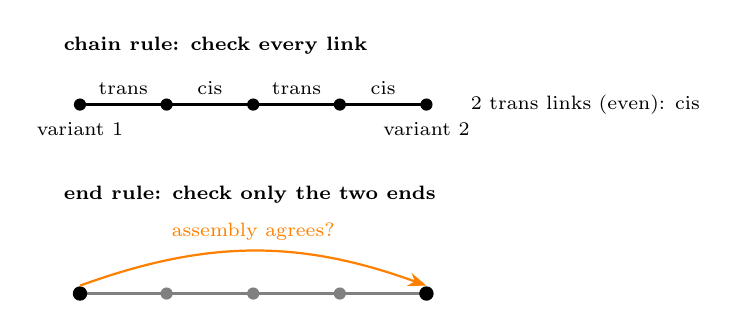
\begin{tikzpicture}[x=1.1cm,font=\scriptsize]
  \node[font=\scriptsize\bfseries,anchor=west] at (-0.3,0.75) {chain rule: check every link};
  \foreach \i/\rel in {0/trans,1/cis,2/trans,3/cis}
    \draw[thick] (\i,0) -- node[above] {\rel} (\i+1,0);
  \foreach \i in {0,...,4} \fill (\i,0) circle (2.2pt);
  \node[below] at (0,-0.1) {variant 1}; \node[below] at (4,-0.1) {variant 2};
  \node[anchor=west] at (4.4,0) {2 trans links (even): cis};
  \begin{scope}[yshift=-2.4cm]
  \node[font=\scriptsize\bfseries,anchor=west] at (-0.3,1.25) {end rule: check only the two ends};
  \draw[thick,gray] (0,0) -- (4,0);
  \foreach \i in {0,...,4} \fill[gray] (\i,0) circle (2.2pt);
  \fill (0,0) circle (2.6pt); \fill (4,0) circle (2.6pt);
  \draw[orange,thick,-{Stealth}] (0,0.1) to[bend left=20] node[above]{assembly agrees?} (4,0.1);
  \end{scope}
\end{tikzpicture}
\caption{Two ways to trust a call between two variants of one gene.}
\label{fig:chain}
\end{figure}

\begin{lstlisting}
def chain_call(links):                     # links from variant 1 to variant 2
    trans = sum(1 for l in links if l.relation == "trans")
    return "cis" if trans % 2 == 0 else "trans"

def chain_rule(links, cutoff, assembly):   # Test 8
    return all(trusted(l, cutoff, assembly) for l in links)

def end_rule(v1, v2, phaser, assembly):    # checked on NA12878 in Test 12
    return assembly.relation(v1, v2) == phaser.relation(v1, v2)
\end{lstlisting}

\paragraph{Without an assembly.} I first used a fixed list of
clinically relevant genes on HG002 Nanopore at 30$\times$: 33{,}055{,}724
site pairs in one gene and at most 100\,kb apart. With the plain per-type
cutoffs, the chain could be trusted at $10^{-2}$ for 53 per cent of pairs up
to 1\,kb apart but only 0.3 per cent of pairs 10 to 100\,kb apart (WhatsHap),
mostly because untrusted indel links break the chain. On HG002 HiFi, 3.7
(WhatsHap) and 14.3 (LongPhase) per cent of gene pairs were answered, with
no sampled answer above its bound in 60 cells.

\paragraph{Test 8 (chain rule).} All site pairs in one clinically relevant
gene, at most 100\,kb apart, on NA12877 and HG005, with Test 7's cutoffs.
To check the promise, one answered pair per gene was picked by a hash that
ignores the phase, in 8 cells (level $0.05/8$). No cell broke (0 wrong picks
of about 2{,}200 to 2{,}400 genes in seven cells, 1 in the eighth). The
assembly rule makes many more pairs answerable (Figure~\ref{fig:genebars}).


\begin{figure}[h]
\centering
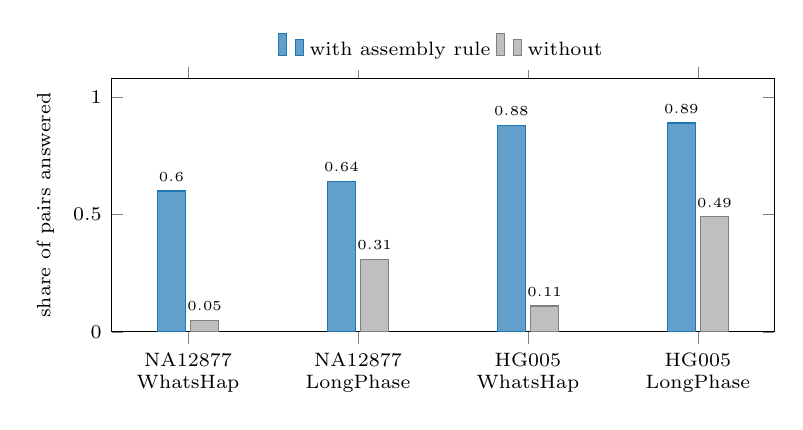
\begin{tikzpicture}
\begin{axis}[ybar,width=10cm,height=4.8cm,bar width=10pt,
  symbolic x coords={a,b,c,d},xtick=data,
  xticklabels={{NA12877\\WhatsHap},{NA12877\\LongPhase},{HG005\\WhatsHap},{HG005\\LongPhase}},
  xticklabel style={align=center},
  ymin=0,ymax=1.08,ylabel={share of pairs answered},enlarge x limits=0.15,
  legend style={font=\scriptsize,draw=none,at={(0.5,1.03)},anchor=south,legend columns=2},
  nodes near coords,nodes near coords style={font=\tiny,/pgf/number format/fixed},
  tick label style={font=\scriptsize},label style={font=\scriptsize}]
\addplot[fill=keep!70,draw=keep] coordinates {(a,0.60) (b,0.64) (c,0.88) (d,0.89)};
\addplot[fill=gray!50,draw=gray] coordinates {(a,0.05) (b,0.31) (c,0.11) (d,0.49)};
\legend{with assembly rule, without}
\end{axis}
\end{tikzpicture}
\caption{Gene pairs answered at a $10^{-2}$ target (Test 8).}
\label{fig:genebars}
\end{figure}

The gain is at long range: WhatsHap on NA12877 answered 55 per cent of pairs
10 to 100\,kb apart, against 0.7 per cent without the rule.

\begin{figure}[h]
\centering
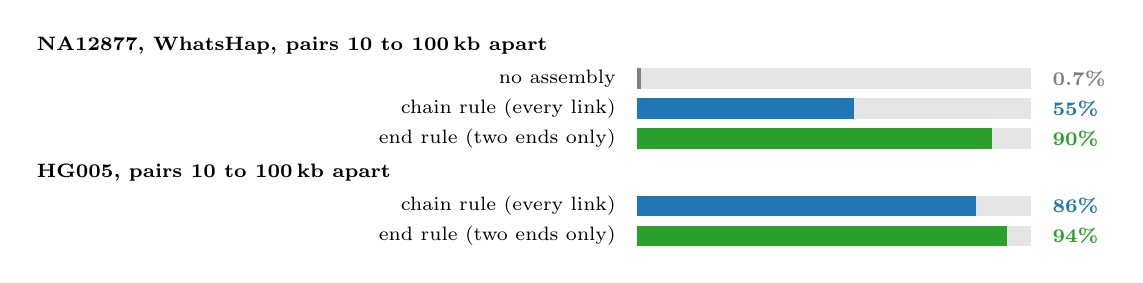
\begin{tikzpicture}[x=5cm]
  \node[anchor=west,font=\scriptsize\bfseries] at (-1.55,0.42) {NA12877, WhatsHap, pairs 10 to 100\,kb apart};
  \failbar{0}{no assembly}{0.007}{0.7\%}{gray}
  \failbar{-0.38}{chain rule (every link)}{0.55}{55\%}{keep}
  \failbar{-0.76}{end rule (two ends only)}{0.90}{90\%}{good}
  \node[anchor=west,font=\scriptsize\bfseries] at (-1.55,-1.2) {HG005, pairs 10 to 100\,kb apart};
  \failbar{-1.62}{chain rule (every link)}{0.86}{86\%}{keep}
  \failbar{-2.0}{end rule (two ends only)}{0.94}{94\%}{good}
\end{tikzpicture}
\caption{Share of far gene pairs that get a trusted answer. Asking the
assembly about the two ends, instead of every link between them, answers
most far pairs.}
\label{fig:farpairs}
\end{figure}

\paragraph{End rule.} With the chain rule, one link the assembly cannot
call blocks the whole chain, although the doctor only needs the answer
between the two ends. Asking the assembly only about the two ends raised far pairs on
NA12877 from 55 to 90 per cent answered, and on HG005 from 86 to 94 per
cent, with no broken cell (checked with one pair per pool person, gene,
distance bin and region type, picked by hash).
Asking both phasers and the assembly to agree at the ends kept the share
and cut wrong answered pairs on NA12877 from 498 (WhatsHap) and 2{,}081
(LongPhase) to 88. Then 82 per cent of NA12877's 2{,}672 genes and 97 per
cent of HG005's 2{,}498 had an answered pair. Reads that span both ends,
used in place of the assembly, answered only 7 to 15 per cent of pairs
beyond 10\,kb: few reads are that long. On NA12878 (Test 12) the end rule
answered 90 and 89 per cent. At $10^{-3}$ nothing far is answered: the
pool's 11{,}500 picks per group allow at most 5 wrong.

\paragraph{Limit.} Genes with a near-identical copy stay \enquote{not sure}: PMS2
(inherited bowel cancer) had 20 of 2{,}346 pairs answered with the chain rule
(78 with the end rule) on NA12877; CYP11B2 and OTOA had none. In these
genes the method gives almost no answers, and so makes almost no errors.

%=====================================================================
\section{Errors outside the benchmark region}\label{sec:outside}
%=====================================================================

Official benchmarks score phasing only inside a \enquote{confident} region, where
the answer key is believed to be reliable. I also scored outside it. HG002
HiFi at 30$\times$, scored against the Q100 key inside and outside GIAB's
v5.0q region:

\begin{center}
\small
\begin{tabular}{@{}lrrrrr@{}}
\toprule
 & \multicolumn{2}{c}{inside} & \multicolumn{2}{c}{outside} & errors\\
phaser & links & wrong & links & wrong & outside\\
\midrule
WhatsHap & 2{,}556{,}197 & 12{,}655 & 192{,}393 & 14{,}052 & 53\%\\
LongPhase & 2{,}515{,}697 & 1{,}111 & 200{,}420 & 16{,}655 & 94\%\\
\bottomrule
\end{tabular}
\end{center}

\begin{figure}[h]
\centering
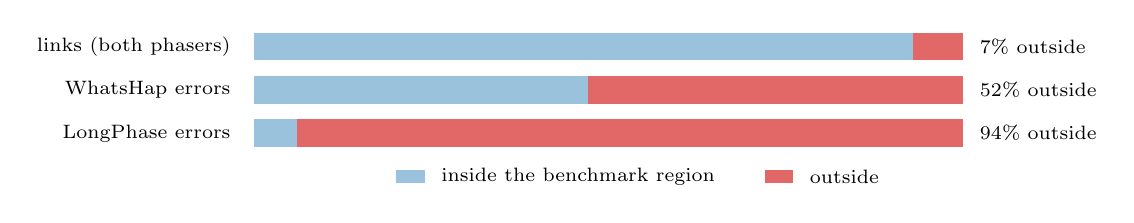
\begin{tikzpicture}[x=9cm,y=0.55cm,font=\scriptsize]
  \foreach \y/\l/\o in {2/links (both phasers)/0.07,1/WhatsHap errors/0.53,0/LongPhase errors/0.94} {
    \node[anchor=east] at (-0.02,\y) {\l};
    \fill[keep!45] (0,\y-0.32) rectangle (1-\o,\y+0.32);
    \fill[bad!70] (1-\o,\y-0.32) rectangle (1,\y+0.32);
    \pgfmathtruncatemacro{\pc}{100*\o}
    \node[anchor=west] at (1.01,\y) {\pc\% outside};}
  \fill[keep!45] (0.2,-1.15) rectangle (0.24,-0.85); \node[anchor=west] at (0.25,-1) {inside the benchmark region};
  \fill[bad!70] (0.72,-1.15) rectangle (0.76,-0.85); \node[anchor=west] at (0.77,-1) {outside};
\end{tikzpicture}
\caption{HG002 HiFi: only 7 per cent of links lie outside the benchmark
region, but most of the errors do.}
\label{fig:outside}
\end{figure}

Outside links are 7 per cent of links but hold 53 and 94 per cent of the
errors (Figure~\ref{fig:outside}); the worst is \grp{lowmap} outside the region, with 13.9 and 24.2 per
cent of links wrong. Cutoffs tuned inside broke outside in 11 of 25 cells.
Chromosome 20, held back, agreed, and a separate recount from the VCF files
alone reproduced every count. HG005 (Test
10): outside links are 27 per cent and hold 95.6 and 94.1 per cent of errors.
NA12878 (Test 12): 91.4 and 84.8 per cent, with error per link 41 and 23
times higher outside.

Outside the region the key is less certain, and for HG002 and HG005 it is an
assembly, so an \enquote{error} there is a disagreement. I made two checks.
NA12878's key comes from the family and shows the same pattern. The parents
also give a third opinion. Parent labels (Section~\ref{sec:parents}) agreed with the
assembly inside the region 96.8 and 95.5 per cent of the time. Corrected for
that, the share of outside disputes that are the phaser's mistake was 0.84
(WhatsHap) and 0.72 (LongPhase) on HG002, 0.94 and 0.64 on HG005, all with
95 per cent lower bounds above 0.5. The labels reach only 2 to
15 per cent of the disputes, and the easier ones. So I claim only that a
benchmark scored inside the region sees a small part of the errors.

\paragraph{Causes of the errors.} For each wrong link I checked whether a
perfect solver would have got it right: whether the exact MEC optimum over a
window of 10 sites on each side, with reads kept as WhatsHap keeps them,
prefers the true answer.

\begin{itemize}
\item The reads support the error in 72.6 per cent of WhatsHap's wrong links
  outside the region, and in 58.9 per cent over the 39 HPRC people.
\item A better solver would fix 18.1 per cent of WhatsHap's outside errors,
  and 29.6 per cent over the HPRC people.
\item No read spans the link in 62.2 per cent of LongPhase's outside errors:
  LongPhase links sites that WhatsHap's reads do not bridge.
\end{itemize}

So most hard-region errors are backed by the reads themselves. A better
solver would not fix them, and a score built from counting reads cannot
catch them. The next section looks for other signs in the reads.

%=====================================================================
\section{Flags from the sample's own reads}\label{sec:flags}
%=====================================================================

When the reads back an error, other features of the reads can still look
wrong. I tried four flags, each computed from the sample alone, on HG002
HiFi:

\begin{itemize}
\item Allele balance. At a true heterozygous site about half the reads show
  each letter; a binomial $-\log_{10}p$ measures how far off the site is.
\item Local solver cost: the extra weighted MEC cost of the exact solution
  in a window of two sites on each side, per read.
\item Depth against the chromosome median, since a copied region collects
  extra reads.
\item Excess of 31-letter words: how many more times the local 31-mers occur
  in the reads than one copy would give.
\end{itemize}

Flags and their cutoffs were tuned per region type on the odd-numbered
chromosomes, flagging at most 9 per cent of links. Flagged links get \enquote{not
sure}, and Learn then Test runs on the rest (the eligible-links fact). The
even-numbered chromosomes were kept aside for checking. On even chromosomes, in
\grp{tandem}, the flags caught 79.5 per cent of wrong links and 98.8 per
cent of the 165 confidently wrong ones (every spanning read wrong, at least
10 reads). The three \grp{tandem} cells that had trusted nothing at
$10^{-3}$ now passed, and no flagged cell broke (0 of 90). Allele balance
and solver cost carried the signal (Figure~\ref{fig:flags}).

\begin{figure}[h]
\centering
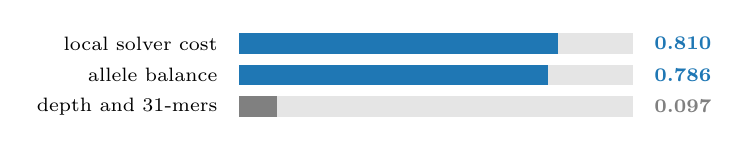
\begin{tikzpicture}[x=5cm]
  \failbar{0}{local solver cost}{0.810}{0.810}{keep}
  \failbar{-0.4}{allele balance}{0.786}{0.786}{keep}
  \failbar{-0.8}{depth and 31-mers}{0.097}{0.097}{gray}
\end{tikzpicture}
\caption{Share of wrong \grp{tandem} links each flag catches on its own
(recall).}
\label{fig:flags}
\end{figure}

The same settings, moved unchanged to HG001 Nanopore, caught
76.7 per cent and again made \grp{tandem} pass. In \grp{segdup} and
\grp{lowmap} the flags caught 78 to 84 per cent of wrong links, but
\grp{segdup} still could not pass: HG002's odd chromosomes have about 1{,}650
\grp{segdup} stretches, below the floor of 2{,}995.

%=====================================================================
\section{Labels from parents}\label{sec:parents}
%=====================================================================

\paragraph{A new batch needs its own labels.} Pooling six Nanopore people and
holding each out in turn, all 23 broken cells (of 1{,}512) had HG002's 2025
reads held out; the pool was mostly older data. So a new sequencing batch
can break the promise on its own. With HG002's 2025 reads as the new batch,
Learn then Test on $k$ sampled HG002 stretches
passed no region type at $10^{-3}$ for $k=$ 300, 1{,}000 or 3{,}000 (20 seeds
each), as the floor requires, since each type then has fewer than 2{,}995.
With all about 11{,}800 easy stretches of HG002's odd chromosomes it passed
\grp{easy} and \grp{difficult} in 4 of 4 cells. Mixing the pool with HG002's
stretches broke cells until HG002's own stretches dominated.

So a new batch needs about 3{,}000 labelled stretches of that batch. A
patient has no answer key, but parents sequenced in the same batch can give
labels (Figure~\ref{fig:trio}):

\begin{figure}[h]
\centering
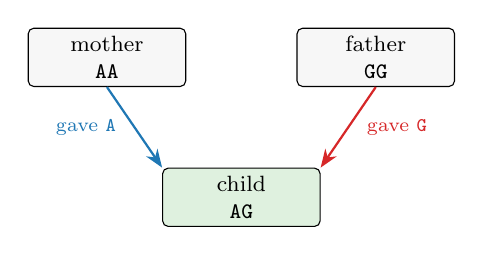
\begin{tikzpicture}[node distance=4mm and 14mm,
  pp/.style={box,minimum width=20mm}]
  \node[pp] (m) {mother\\\dna{AA}};
  \node[pp,right=of m] (f) {father\\\dna{GG}};
  \node[pp,fill=good!15,below=14mm of $(m)!0.5!(f)$] (c) {child\\\dna{AG}};
  \draw[arr,hapA] (m.south) -- node[left=3pt,font=\scriptsize]{gave \dna{A}} (c.north west);
  \draw[arr,hapB] (f.south) -- node[right=3pt,font=\scriptsize]{gave \dna{G}} (c.north east);
\end{tikzpicture}
\caption{The mother has only \dna{A}, so the child's \dna{A} came from her.
Two such sites next to each other label the link between them.}
\label{fig:trio}
\end{figure}

\begin{center}
\small
\begin{tabular}{@{}llll@{}}
\toprule
child & mother & father & child's \dna{A} came from\\
\midrule
\dna{AG} & \dna{AA} & \dna{GG} & the mother\\
\dna{AG} & \dna{AG} & \dna{AG} & unknown\\
\bottomrule
\end{tabular}
\end{center}

If a parent has two identical letters at a site, we know what the child got
from that parent. Two such neighbouring sites give a link label. First I
checked the idea on the HG002 trio's known phase: transmission labels were
wrong only 1.7 times in $10^5$. But parent letters called by Clair3 from one
sequencing run gave labels wrong $2.06\times10^{-4}$ of the time on easy
links, above WhatsHap's own error there ($1.84\times10^{-5}$), so nothing
could pass. Using a site only when two separate runs of each parent agree
cut the label error to $1.33\times10^{-5}$, with 77.6 per cent of links
labelled.

Labelled links are easier: WhatsHap's error on unlabelled \grp{lowmap}
links was $3.8\times10^{-3}$, on labelled ones $7.0\times10^{-5}$. So tuning
on labelled links and testing on all links broke 1 cell (190 bad of
43{,}599 stretches). Following the eligible-links fact, tune and test on
labelled links only and say \enquote{not sure} elsewhere: then no cell of 108
broke on HG002, \grp{easy} passed $10^{-3}$ in 6 of 6 cells,
and 77.4 per cent of all easy links were trusted.

\paragraph{Test 9.} HG005 Nanopore, labels from two runs each of its parents
HG006 and HG007; tuned on labelled links of odd chromosomes, checked on even
ones. No cell broke (0 of the 90 cells with links; smallest $p=0.44$).
\grp{easy} passed $10^{-3}$ everywhere, with 99.3 per cent of even-chromosome
easy links trusted; \grp{difficult}, \grp{lowmap} and \grp{tandem} passed
$10^{-3}$ in every cell too, \grp{segdup} only $3\times10^{-3}$. The
trusted share is too high to carry over: HG005's key comes from the same
parents, so nearly all scored links were labelled. The test shows that the
promise holds on a second family and batch. It does not show how many links
a new family would get trusted.

%=====================================================================
\section{Five predictions on NA12878}\label{sec:na12878}
%=====================================================================

Test 12 checks the answer-key explanation and the end rule on a new
person: NA12878 (HG001), the family's mother, whose HiFi reads had not been
used anywhere before. Five predictions were made before her data were
phased. Her data: phasing at 30, 20 and 10$\times$ with WhatsHap and
LongPhase (108 cells), and an assembly from about 30$\times$ of her reads.
Her key is the four-generation family key, with no assembly in it, so it
does not share the weakness of the HPRC keys.

All five held:

\begin{enumerate}
\item Test 6's pooled cutoffs break on all links. 31 of 108 cells broke.
\item The same cutoffs hold on links her family key labels. 0 of 108 broke,
  against 20 for random links.
\item Test 7's assembly rule holds, and \grp{segdup} passes $10^{-3}$. 0 of
  36 cells broke, and 78 per cent of \grp{segdup} links were trusted.
\item The end rule answers at least 70 per cent of far gene pairs. 0 of 4
  cells broke, and 90 and 89 per cent were answered.
\item Most errors lie outside the benchmark region. 91 and 85 per cent did.
\end{enumerate}

\enquote{Links her family key labels}: her assembly relates the pair the same way
as transmission from her parents NA12891 and NA12892. Prediction 1's 31
breaks: 13 \grp{segdup}, 11 \grp{lowmap}, 6 \grp{indel}, 1 \grp{tandem}.
Predictions 1 and 2 are the main check: the answer-key explanation
predicted both the failure and where it disappears, on someone new.

\paragraph{Caveats.} She is the mother of the children in the pools of
Predictions 3 and 4, and bad stretches are shared between relatives, so those
two are not fully independent checks. Predictions 1 and 2 use a
pool with nobody from her family. Not reached: \grp{segdup} at
$3\times10^{-4}$, gene calls at $10^{-3}$.

%=====================================================================
\section{One rule that explains the results}\label{sec:rule}
%=====================================================================

\begin{center}
\fbox{\begin{minipage}{0.8\textwidth}\centering
A promise holds on the links its answer key came from.\\
Tune and test on links chosen by the same rule, and report the rule.
\end{minipage}}
\end{center}

I sorted all 37 promise tests of the project by whether the test links
were chosen the same way as the tuning links.

\paragraph{Tuning and test links chosen the same way.} No cell broke.
\begin{itemize}
\item HG002 with cheaper basecalling (Test 2): 0 of 18 cells broke; HG001 on
  GIAB's own sites: 0 of 18.
\item Relatives with the same family key (Test 3): easy 0 of 126; hard 0 of
  540.
\item Gene calls: chain rule (Test 8) 0 of 8; end rule 0 of 8.
\item Pooled cutoffs on key links: family 0 of 540; 19 people (Test 11) 0 of
  2{,}052.
\item Assembly rule (Test 7): 0 of 62; on NA12878 (Test 12): 0 of 36.
\item Parent labels: HG002 0 of 108; HG005 (Test 9) 0 of 90.
\end{itemize}

\paragraph{Test links reaching beyond the tuning labels.} Cells broke.
\begin{itemize}
\item One cutoff, HG001, 2017 key (Test 2): 18 of 18 broke; against the
  family key: 12 of 18.
\item HG001 hard types, family key beyond GIAB's regions (Test 4): 2 of 90.
\item Parent labels, tested on all links: 1 of 108.
\item Pooled cutoffs on all links: family (Test 6) 163 of 540; 19 people
  (Test 11) 1{,}221 of 2{,}052.
\item NA12878, all links (Test 12): 31 of 108.
\item Tuned inside the benchmark region, tested outside (HG002): 11 of 25.
\end{itemize}

Every break came from test links beyond the tuning population. This
breaks Learn then Test's assumption (1), and the break is easy to miss when
the answer key is itself a selection of links. One exception has a different
cause: a new sequencing batch can break
the promise alone (all 23 of 1{,}512 broken cells, when six Nanopore people
were pooled and each held out in turn, had HG002's 2025 reads held out),
which is why the floor in Section~\ref{sec:floor} is stated per batch. The
rule predicts whether a promise breaks. It does not predict the size of the
break.

%=====================================================================
\section{Ideas that did not work}\label{sec:honest}
%=====================================================================

Each idea was judged by a pass rule set before it was tried. The
read-selection ideas are in Section~\ref{sec:whatshap}.

\begin{itemize}
\item A learned score (gradient boosting on 22 read features, and a neural
  score) raised WhatsHap's trusted \grp{tandem} share at $10^{-3}$ from 0 to
  86 per cent on HG002 Nanopore, but \grp{segdup} passed nowhere.
\item With the complete T2T reference (CHM13), 25 of 27 confidently wrong
  links stayed wrong.
\item Telling the parent of origin from methylation failed: phase blocks
  carried the parent label to the wrong parent for 16.2 per cent of 198{,}729
  sites near imprinted regions~\cite{akbari2022}. Trusted blocks had 0 wrong
  of 586, but the phaser was right on all 586 too.
\item Labels from two siblings without parents had an error of
  $2.73\times10^{-2}$, and $2.82\times10^{-3}$ after a repair, where
  $10^{-4}$ was needed. Two siblings cannot tell unshared stretches from
  shared ones.
\item Labels from NA12878's parents' called letters failed their rule, and so
  did the planned repair.
\item Estimating answer-key errors without a gold standard, with a
  four-source latent-class fit on NA12878, gave different answers on odd and
  even chromosomes. No key reached $10^{-3}$ in a hard region.
\item Bins where HG002 made errors raised other people's error only 0.5 to
  2.1 times (HG002's own other reads: 4.6 to 21). Each person's errors sit
  in different places.
\item A planner for pool size predicted pass rates right in 13 of 51 cells,
  where the rule needed 80 per cent.
\item HiFi and Nanopore did not work as second opinions for each other: on
  wrong \grp{segdup} links the other platform made the same error 39 to 59
  per cent of the time (the rule needed under 20 per cent). Both use the
  same reference.
\item Asking three methods to agree on gene calls at $10^{-3}$ gave 6 wrong
  picks where the pool allowed 5.
\end{itemize}


%=====================================================================
\section{Limits}\label{sec:limits}
%=====================================================================

\begin{itemize}
\item Optimal selection helped only at cap 3; most selection results are on
  HG002 (HG005 replicates HiFi), only single-letter sites inside the
  benchmark region were scored, and every lower-depth sample used one seed.
\item The flags, the parent check on outside errors, and the error-cause
  breakdown were measured on one or two people, not yet tested on new
  people.
\item 100\,kb stretches are not independent in hard regions (bad ones clump
  in 181 of 576 tests); 200 and 300\,kb stretches changed no decision in 360
  cells.
\item The assembly rule needs HiFi reads at full depth and a whole-genome
  assembly for every person.
\item NA12877 and NA12878 are related to the pool; HG005, the unrelated test,
  has no indel key; the 19 HPRC people's scoring key is an assembly.
\end{itemize}

\paragraph{Next steps.}
\begin{enumerate}
\item A second opinion without an assembly, for Nanopore and low coverage.
\item Duplicated genes like PMS2: gene-aware assembly or targeted reads.
\item A test of the parent check on outside-region errors on new people.
\item A test of the read-derived flags
  (Section~\ref{sec:flags}) on a new person.
\item An unrelated person with an indel key; parent-label coverage against a
  key not built from parents.
\item Gene-panel calls checked against families.
\end{enumerate}

%=====================================================================
\section{Conclusion}\label{sec:summary}
%=====================================================================

\begin{enumerate}
\item The best choice of reads is a min-cost flow. WhatsHap's shipped greedy
  rule gets 93 to 96 per cent of the way there, and it differs from the rule
  in its paper. Inside \code{whatshap phase}, the best choice cut errors by
  42 per cent when only 3 reads are kept, and made no clear difference at
  the default cap of 15.
\item One cutoff per region type, chosen by Learn then Test, kept its
  promise in 582 of 582 easy-region test cells across three ancestries,
  while trusting over 99.5 per cent of links.
\item One person never gives enough data for a promise in duplications. Six
  people plus an agreeing assembly held on three new people and trusted 78
  to 96 per cent of duplication links.
\item An answer key that labels only where two methods agree picks the easy
  links, and cutoffs tuned on it hold only on links like those. This was
  confirmed on 19 new people and on NA12878.
\item With the assembly, about 90 per cent of far gene pairs get an answer.
  Benchmarks scored inside the confident region miss most errors, and most
  hard-region errors are backed by the reads. Flags from a sample's own
  reads make tandem repeats pass, and labels from parents work for a new
  sequencing batch.
\end{enumerate}

\begin{table}[h]
\centering
\small
\begin{tabular}{@{}p{9.2cm}ccc@{}}
\toprule
result & proved & \makecell{tested on\\unseen data} & \makecell{measured on\\data seen}\\
\midrule
the best choice of reads is a min-cost flow & \ding{51} & & \\
WhatsHap's greedy keeps 93 to 96\% of the best weight & & & \ding{51}\\
best choice cuts errors 42\% at cap 3, none at cap 15 (Test 1) & & \ding{51} & \\
one genome-wide cutoff breaks on a new person (Test 2) & & \ding{51} & \\
per-type cutoffs hold in all 582 easy cells (Tests 3 to 6) & & \ding{51} & \\
one person is never enough data for duplications & \ding{51} & & \\
assembly rule holds on three new people (Tests 7, 12) & & \ding{51} & \\
promises break because the answer key covers easy links & & \ding{51} & \ding{51}\\
end rule answers about 90\% of far gene pairs (Test 12) & & \ding{51} & \ding{51}\\
most errors lie outside the benchmark region (Tests 10, 12) & & \ding{51} & \ding{51}\\
parent labels work for a new batch (Test 9) & & \ding{51} & \ding{51}\\
most hard-region errors are backed by the reads & & & \ding{51}\\
flags from a sample's own reads make tandem repeats pass & & & \ding{51}\\
one rule explains every broken promise (Section~\ref{sec:rule}) & & & \ding{51}\\
\bottomrule
\end{tabular}
\caption{How strong each main result is. A tick in both of the last two
columns means the result was found on data already seen and then checked on
unseen data. The rule of Section~\ref{sec:rule} was stated after most tests;
the two tests scored after it (Tests 11 and 12) fit it.}
\label{tab:strength}
\end{table}

%=====================================================================
\section{Glossary}\label{sec:glossary}
%=====================================================================

\begin{description}[leftmargin=0pt,itemsep=1pt,font=\normalfont\bfseries]
\item[Allele.] One of the letters found at a variant position.
\item[Answer key.] A phase believed to be correct, used to count a phaser's
  errors (also called a truth set).
\item[Assembly.] Both copies of a person's genome rebuilt directly from the
  reads, without the reference (here with hifiasm and dipcall).
\item[Base quality.] The sequencer's confidence that a letter was read
  correctly.
\item[Block (phase block).] A run of variants phased together; the phaser
  gives no link between blocks.
\item[Cap.] The largest number of reads WhatsHap keeps over any position.
\item[Cell.] One combination of test person, coverage, phaser, error target
  and region type, scored on its own.
\item[Chromosome.] One of the 23 pieces the genome is split into; everyone
  has two copies of each.
\item[Cis / trans.] Two variants on the same copy (cis) or on different
  copies (trans).
\item[Coverage (depth).] How many reads cover a position on average.
\item[Dynamic program.] A method that solves a problem step by step, here
  position by position, while keeping every partial answer that could still
  be best.
\item[Greedy rule.] A quick rule that takes the best-looking choice at each
  step without looking ahead.
\item[Heterozygous site.] A position where the two copies have different
  letters.
\item[Learn then Test.] A statistical method that picks a cutoff so that the
  error rate among accepted answers is below a target, with a stated
  confidence.
\item[Link.] The cis or trans answer between two neighbouring heterozygous
  sites.
\item[Long read.] A read of 10{,}000 letters or more (PacBio HiFi, Oxford
  Nanopore).
\item[MEC (minimum error correction).] Choosing the two copies that need the
  fewest letter changes to fit all reads.
\item[Min-cost flow.] A network problem that sends units through arcs at the
  lowest total cost; it solves the read choice exactly.
\item[N50.] Half of the phased sequence lies in blocks at least this long.
\item[Phasing.] Working out which letters sit on the same copy of a
  chromosome.
\item[Read.] A piece of DNA read by a sequencer.
\item[Reference genome.] A standard human genome that reads are matched
  against.
\item[Region type.] One of six classes of the genome by how hard it is to
  phase (Section~\ref{sec:regions}).
\item[Segmental duplication.] A long stretch of DNA that appears in more
  than one place in the genome.
\item[Sign test.] A test that treats each disagreement between two methods
  as a coin toss and asks whether one side wins too often.
\item[Stretch.] A 100\,kb window of a chromosome, the unit the promise
  counts.
\item[Switch error.] A wrong link.
\item[Variant.] A position where a person's DNA differs from the reference.
\end{description}

\begin{thebibliography}{99}
\footnotesize\setlength{\itemsep}{0pt}\setlength{\parskip}{0pt}
\bibitem{akbari2022} V.~Akbari et al. Genome-wide detection of imprinted
differentially methylated regions using nanopore sequencing. \emph{eLife}
11:e77898, 2022.
\bibitem{bareyehuda2006} R.~Bar-Yehuda, M.~M.~Halld\'orsson, J.~Naor,
H.~Shachnai, I.~Shapira. Scheduling split intervals. \emph{SIAM J. Comput.}
36(1):1--15, 2006.
\bibitem{damaraju2026} N.~Damaraju et al. Determinants of haplotype phasing
accuracy in long-read human genome sequencing. bioRxiv, 2026.
\bibitem{duitama2012} J.~Duitama et al. Fosmid-based whole genome
haplotyping of a HapMap trio child. \emph{Nucleic Acids Res.}
40(5):2041--2053, 2012.
\bibitem{hapcut2} P.~Edge, V.~Bafna, V.~Bansal. HapCUT2: robust and accurate
haplotype assembly for diverse sequencing technologies. \emph{Genome Res.}
27(5):801--812, 2017.
\bibitem{geifman2017} Y.~Geifman, R.~El-Yaniv. Selective classification for
deep neural networks. \emph{NeurIPS} 30, 2017.
\bibitem{shapeit5} R.~J.~Hofmeister, D.~M.~Ribeiro, S.~Rubinacci,
O.~Delaneau. Accurate rare variant phasing of whole-genome and whole-exome
sequencing data in the UK Biobank. \emph{Nat. Genet.} 55(7):1243--1249, 2023.
\bibitem{majidian2020} S.~Majidian, M.~H.~Kahaei, D.~de~Ridder. Minimum error
correction-based haplotype assembly: considerations for long read data.
\emph{PLOS ONE} 15(6):e0234470, 2020.
\bibitem{makinen2015} V.~M\"akinen, V.~Staneva, A.~I.~Tomescu,
D.~Valenzuela, S.~Wilzbach. Interval scheduling maximizing minimum coverage.
\emph{Discrete Appl. Math.} 225:130--135, 2017.
\bibitem{richards2015} S.~Richards et al. Standards and guidelines for the
interpretation of sequence variants (ACMG/AMP). \emph{Genet. Med.}
17(5):405--424, 2015.
\bibitem{vovk2012} V.~Vovk. Conditional validity of inductive conformal
predictors. \emph{Asian Conf. Mach. Learn.}, 2012. arXiv:1209.2673.
\bibitem{arkin1987} E.~M.~Arkin, E.~B.~Silverberg. Scheduling jobs with fixed
start and end times. \emph{Discrete Appl. Math.} 18:1--8, 1987.
\bibitem{berend2005} D.~Berend, L.~Sapir. Monotonicity in Condorcet jury
theorem. \emph{Soc. Choice Welf.} 24(1):83--92, 2005.
\bibitem{carlisle1995} M.~C.~Carlisle, E.~L.~Lloyd. On the $k$-coloring of
intervals. \emph{Discrete Appl. Math.} 59:225--235, 1995.
\bibitem{cheng2021} H.~Cheng, G.~T.~Concepcion, X.~Feng, H.~Zhang, H.~Li.
Haplotype-resolved de novo assembly using phased assembly graphs with
hifiasm. \emph{Nat. Methods} 18:170--175, 2021.
\bibitem{dwarshuis2024} N.~Dwarshuis et al. The GIAB genomic stratifications
resource for human reference genomes. \emph{Nat. Commun.} 15:9029, 2024.
\bibitem{fischer2016} S.~O.~Fischer, T.~Marschall. Selecting reads for
haplotype assembly. bioRxiv 046771, 2016.
\bibitem{hansen2026} N.~F.~Hansen et al. A complete diploid human genome
benchmark for personalized genomics. \emph{Cell} 189(16):4857--4875, 2026.
\bibitem{holt2024} J.~M.~Holt et al. HiPhase: jointly phasing small,
structural, and tandem repeat variants from HiFi sequencing.
\emph{Bioinformatics} 40(2):btae042, 2024.
\bibitem{kronenberg2025} Z.~Kronenberg et al. The Platinum Pedigree: a
long-read benchmark for genetic variants. \emph{Nat. Methods}
22:1669--1676, 2025.
\bibitem{li2018} H.~Li et al. A synthetic-diploid benchmark for accurate
variant-calling evaluation. \emph{Nat. Methods} 15:595--597, 2018.
\bibitem{lin2022} J.-H.~Lin et al. LongPhase: an ultra-fast chromosome-scale
phasing algorithm for small and large variants. \emph{Bioinformatics}
38(7):1816--1822, 2022.
\bibitem{ltt2025} A.~N.~Angelopoulos, S.~Bates, E.~J.~Cand\`es, M.~I.~Jordan,
L.~Lei. Learn then Test: calibrating predictive algorithms to achieve risk
control. \emph{Ann. Appl. Stat.} 19(2), 2025.
\bibitem{martin2016} M.~Martin et al. WhatsHap: fast and accurate read-based
phasing. bioRxiv 085050, 2016.
\bibitem{patterson2015} M.~Patterson et al. WhatsHap: weighted haplotype
assembly for future-generation sequencing reads. \emph{J. Comput. Biol.}
22(6):498--509, 2015.
\bibitem{wilson1927} E.~B.~Wilson. Probable inference, the law of succession,
and statistical inference. \emph{J. Amer. Statist. Assoc.} 22(158):209--212,
1927.
\end{thebibliography}

\end{document}
